\chapter{Persistierung} % (fold)
\label{cha:persistierung}

In den vorangegangen drei Kapiteln wurde die Umsetzung des eigentlichen Werkzeugs beschrieben. Neben der Unterstützung des Modellierungsvorgangs ist aber auch die persistente Speicherung der erstellten Modelle zum Zwecke der Weiterverarbeitung ein hier zu beleuchtender Aspekt. Auf die Persistierung wirken vor allem zwei der in Kapitel XY identifzierten Anforderungen ein. Zum ersten ist die Nachvollziehbarkeit des Modellierungsvorganges sicherzustellen -- dies gilt nicht nur während des Vorgangs selbst, sondern auch danach. Dementsprechend ist sämtliche Information zu persistieren, die zur Wiederherstellung nicht nur des Modells selbst sondern auch der gesamten Modellierungshistorie notwendig ist. Zum zweiten hat die Forderung nach semantischer Offenheit bei der Modellierung auch unmittelbare Auswirkungen auf die Persistierung. Neben dem Modell selbst muss aufgrund dieser Anforderung auch die Bedeutung der verwendeten Modellierungselemente miterfasst und persistiert werden, so dass diese bei der Weiterverarbeitung der Modelle verwendet werden kann.

In diesem Kapitel werden nun aufgrund der eben genannten Forderungen technologische Ansätze identifiziert, beschrieben und schließlich hinsichtlich ihrer Eignung für den konkreten Einsatz beurteilt. Der ausgewählte Ansatz wird im darauf folgenden Abschnitt konzeptuell beschrieben. Die Abbildung der Modelle und der ebenfalls zu persistierenden zusätzlichen Information in ein geeignetes Datenmodell ist Gegenstand des darauf folgenden Abschnitts. Schließlich wird die konkrete technische Umsetzung der Persistierung dargelegt und die dazu notwendigen Software-Module im Detail beschrieben.
 
\section{Möglichkeiten der Persistenzsicherung} % (fold)
\label{sec:möglichkeiten_der_persistenzsicherung}

\begin{itemize}
	\item Serialisierung von Java-Objekten
	\item Relationale Datenbanken
	\item \gls{XML} Topic Maps
\end{itemize}

% section möglichkeiten_der_persistenzsicherung (end)

\section{Topic Maps} % (fold)
\label{sec:topic_maps}

Topic Maps \citep{TMDM08} sind wie bereits in Abschnitt XY beschrieben ein Mittel zur Abbildung von semantischen Netzen. In Topic Maps können beliebige Daten strukutriert aufbereitet und zueinander in Beziehung gesetzt werden. Die Art der zu repräsentierenden Daten ist dabei irrelvant, eine Topic Map trifft keine Aussage über ein den repräsentierten Daten zugrundeliegendes Begriffsystem (sie ist „ontology-agnostic“ \citep{Vatant04}).

Historisch stammen Topic Maps aus dem Bereich der technischen Repräsentation von Thesauri und Indizes \citep{Pepper00} \citep{Rath03}. Aus diesen Bereichen motivieren sich auch die Bausteine einer Topic Map, wenngleich der Verwendung durch diesen Ursprung nicht eingeschränkt wird. Die grundlegenden Elemente einer Topic Map sind „Topics“, „Associations“ und „Occurrences“ (siehe Abbildung \ref{fig:img_Persistenz_TMBasic}). 

\begin{figure}[htbp]
	\centering
		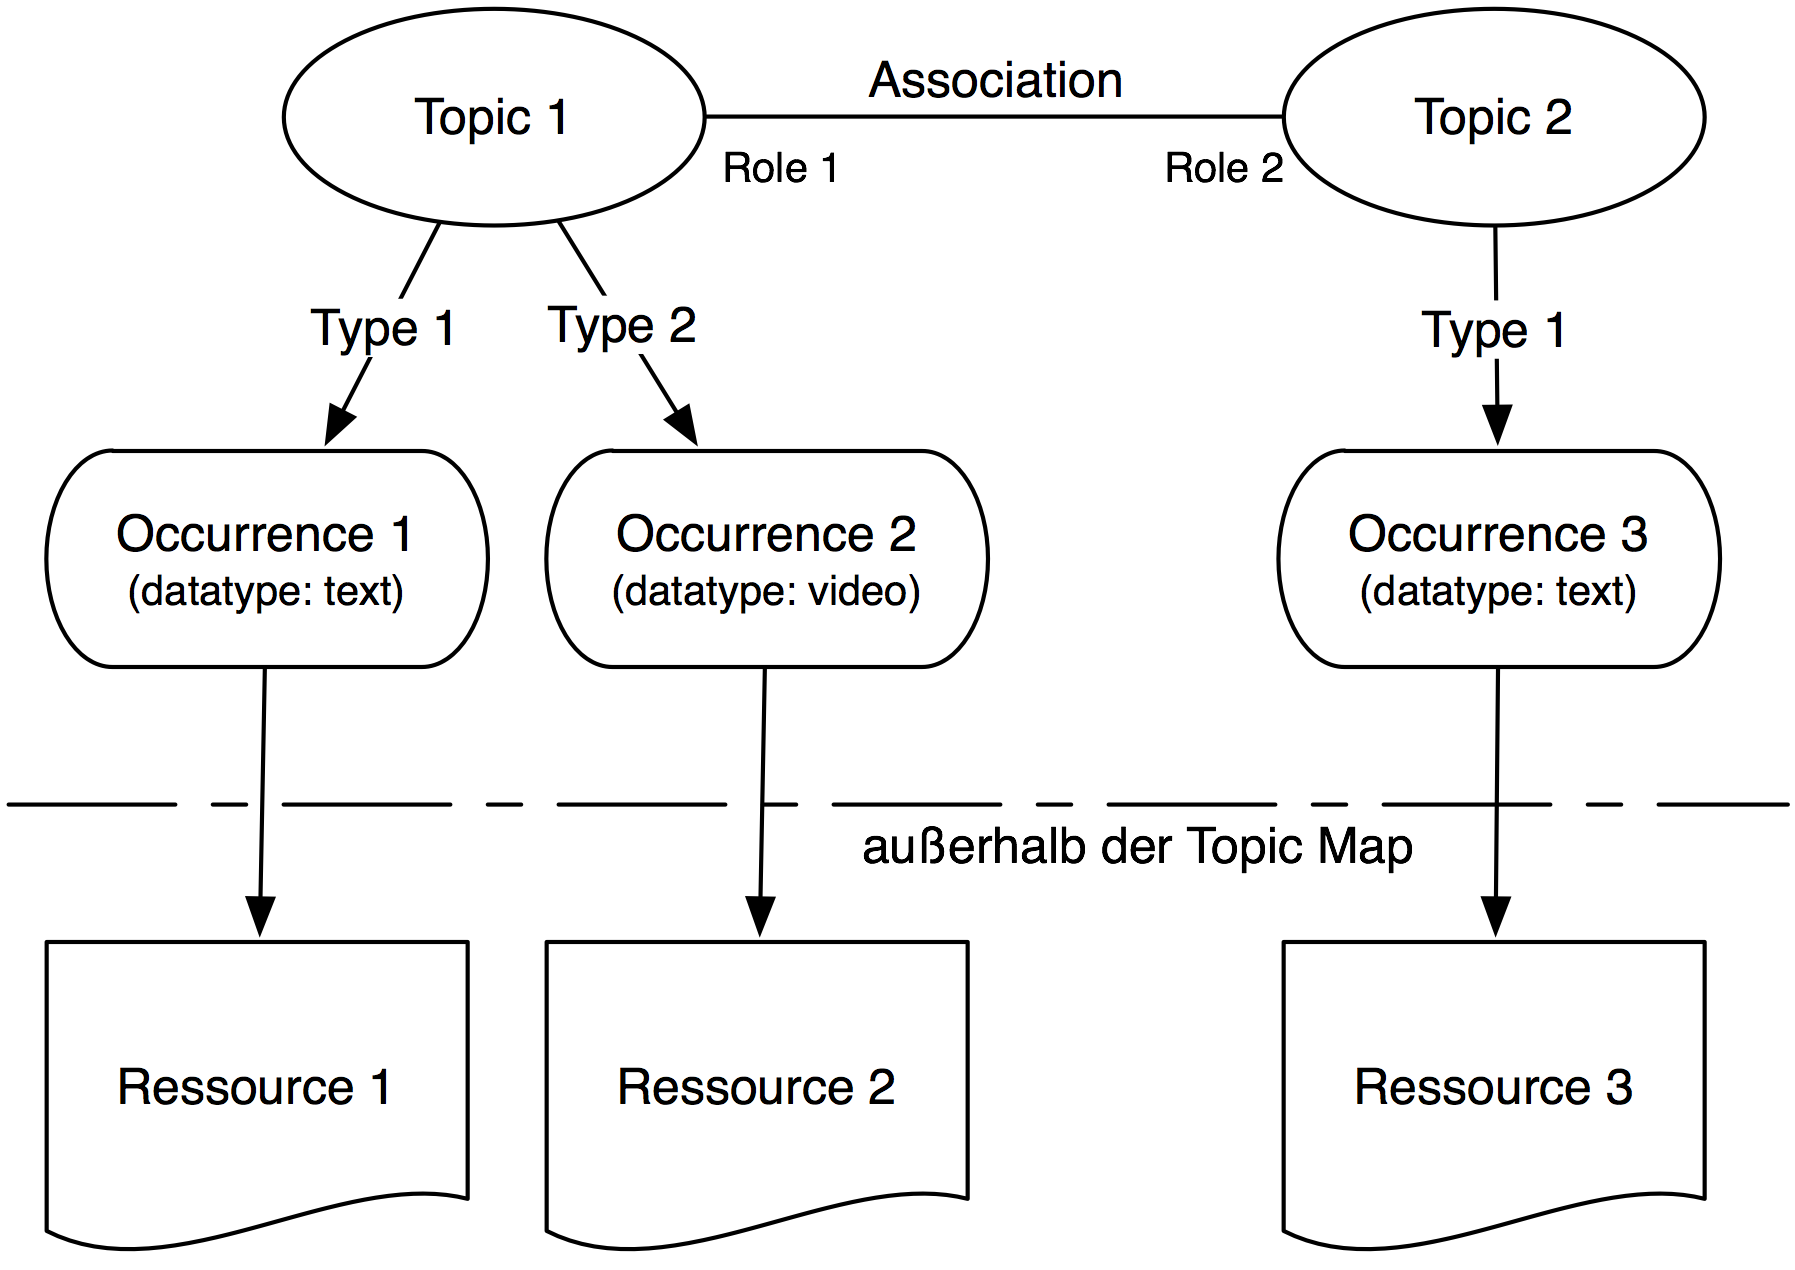
\includegraphics[width=10cm]{img/Persistenz/TMBasic.png}
	\caption{Grundlegende Elemente einer Topic Map}
	\label{fig:img_Persistenz_TMBasic}
\end{figure}

„Topics“ sind stellen Begriffe dar und bilden die Knoten des semantischen Netzes. Ein Topic kann beliebige Information darstellen, repräsentiert aber immer genau ein Phänomen der realen Welt (d.h. zu einem Topic muss es eine Entsprechung außerhalb der Topic Maps geben, die beobachtbar oder beschreibbar ist und auf die die modellierende Person Bezug nehmen will \footnote{„A subject can be anything whatsoever, regardless of whether it exists or has any other specific characteristics, about which anything whatsoever may be asserted by any means whatsoever. In particular, it is anything about which the creator of a topic map chooses to discourse.“ \citep[][S.8]{TMDM08}}). Eine Topic Map ist damit im Sinne von \citet{Stachowiak73} ein diagrammatisches Modell, das einen bestimmten, für den Modellersteller relevanten Ausschnitt der Realität abbildet.

“Associations“ bilden die Beziehungen zwischen Topics ab und stellen damit die Kanten des semantischen Netzes dar. Eine Association verknüpft Topics semantisch miteinander und kann frei mit Bedeutung belegt werden. Die Art der Beziehungen ist also nicht festgelegt und wird wie die Bedeutung der Topics frei gewählt werden. Topics und Associations decken historisch den Bereich der Darstellung von Thesauri ab, in denen Begriffe definiert und zueinanden in Beziehung gesetzt werden. 

Der zweite historische Ursprung von Topic Maps, die Indizes, werden durch das Konstrukt der „Occurences“ abgedeckt. Occurences (“Auftreten“) sind Referenzen aus der Topic Map in die reale Welt. Sie setzen die Topics einer Topic Map in Bezug zu beliebiger referenzierbarer Information (z.B. Dokumente). Im Kontext der eben genannten Indizes, kann eine Topic Map als der mit Querverweisen versehene Index eines Buches verstanden werden, in dem durch die Angabe von Seitenzahlen auf den Text des Buches verwiesen wird. Diese Verweise durch Angabe der Seitenzahlen sind in diesem Zusammenhang die Occurrences.

Die Ansammlung von durch Associations verknüpften und mit Occurrences versehenen Topics bilden eine Topic Map. Darüber hinaus kann in Topic Maps jedoch noch weiterführende Information repräsentiert werden (siehe Abbildung \ref{fig:img_Persistenz_TMFull}), die Gegenstand der folgenden Abschnitte sein werden.

\begin{figure}[htbp]
	\centering
		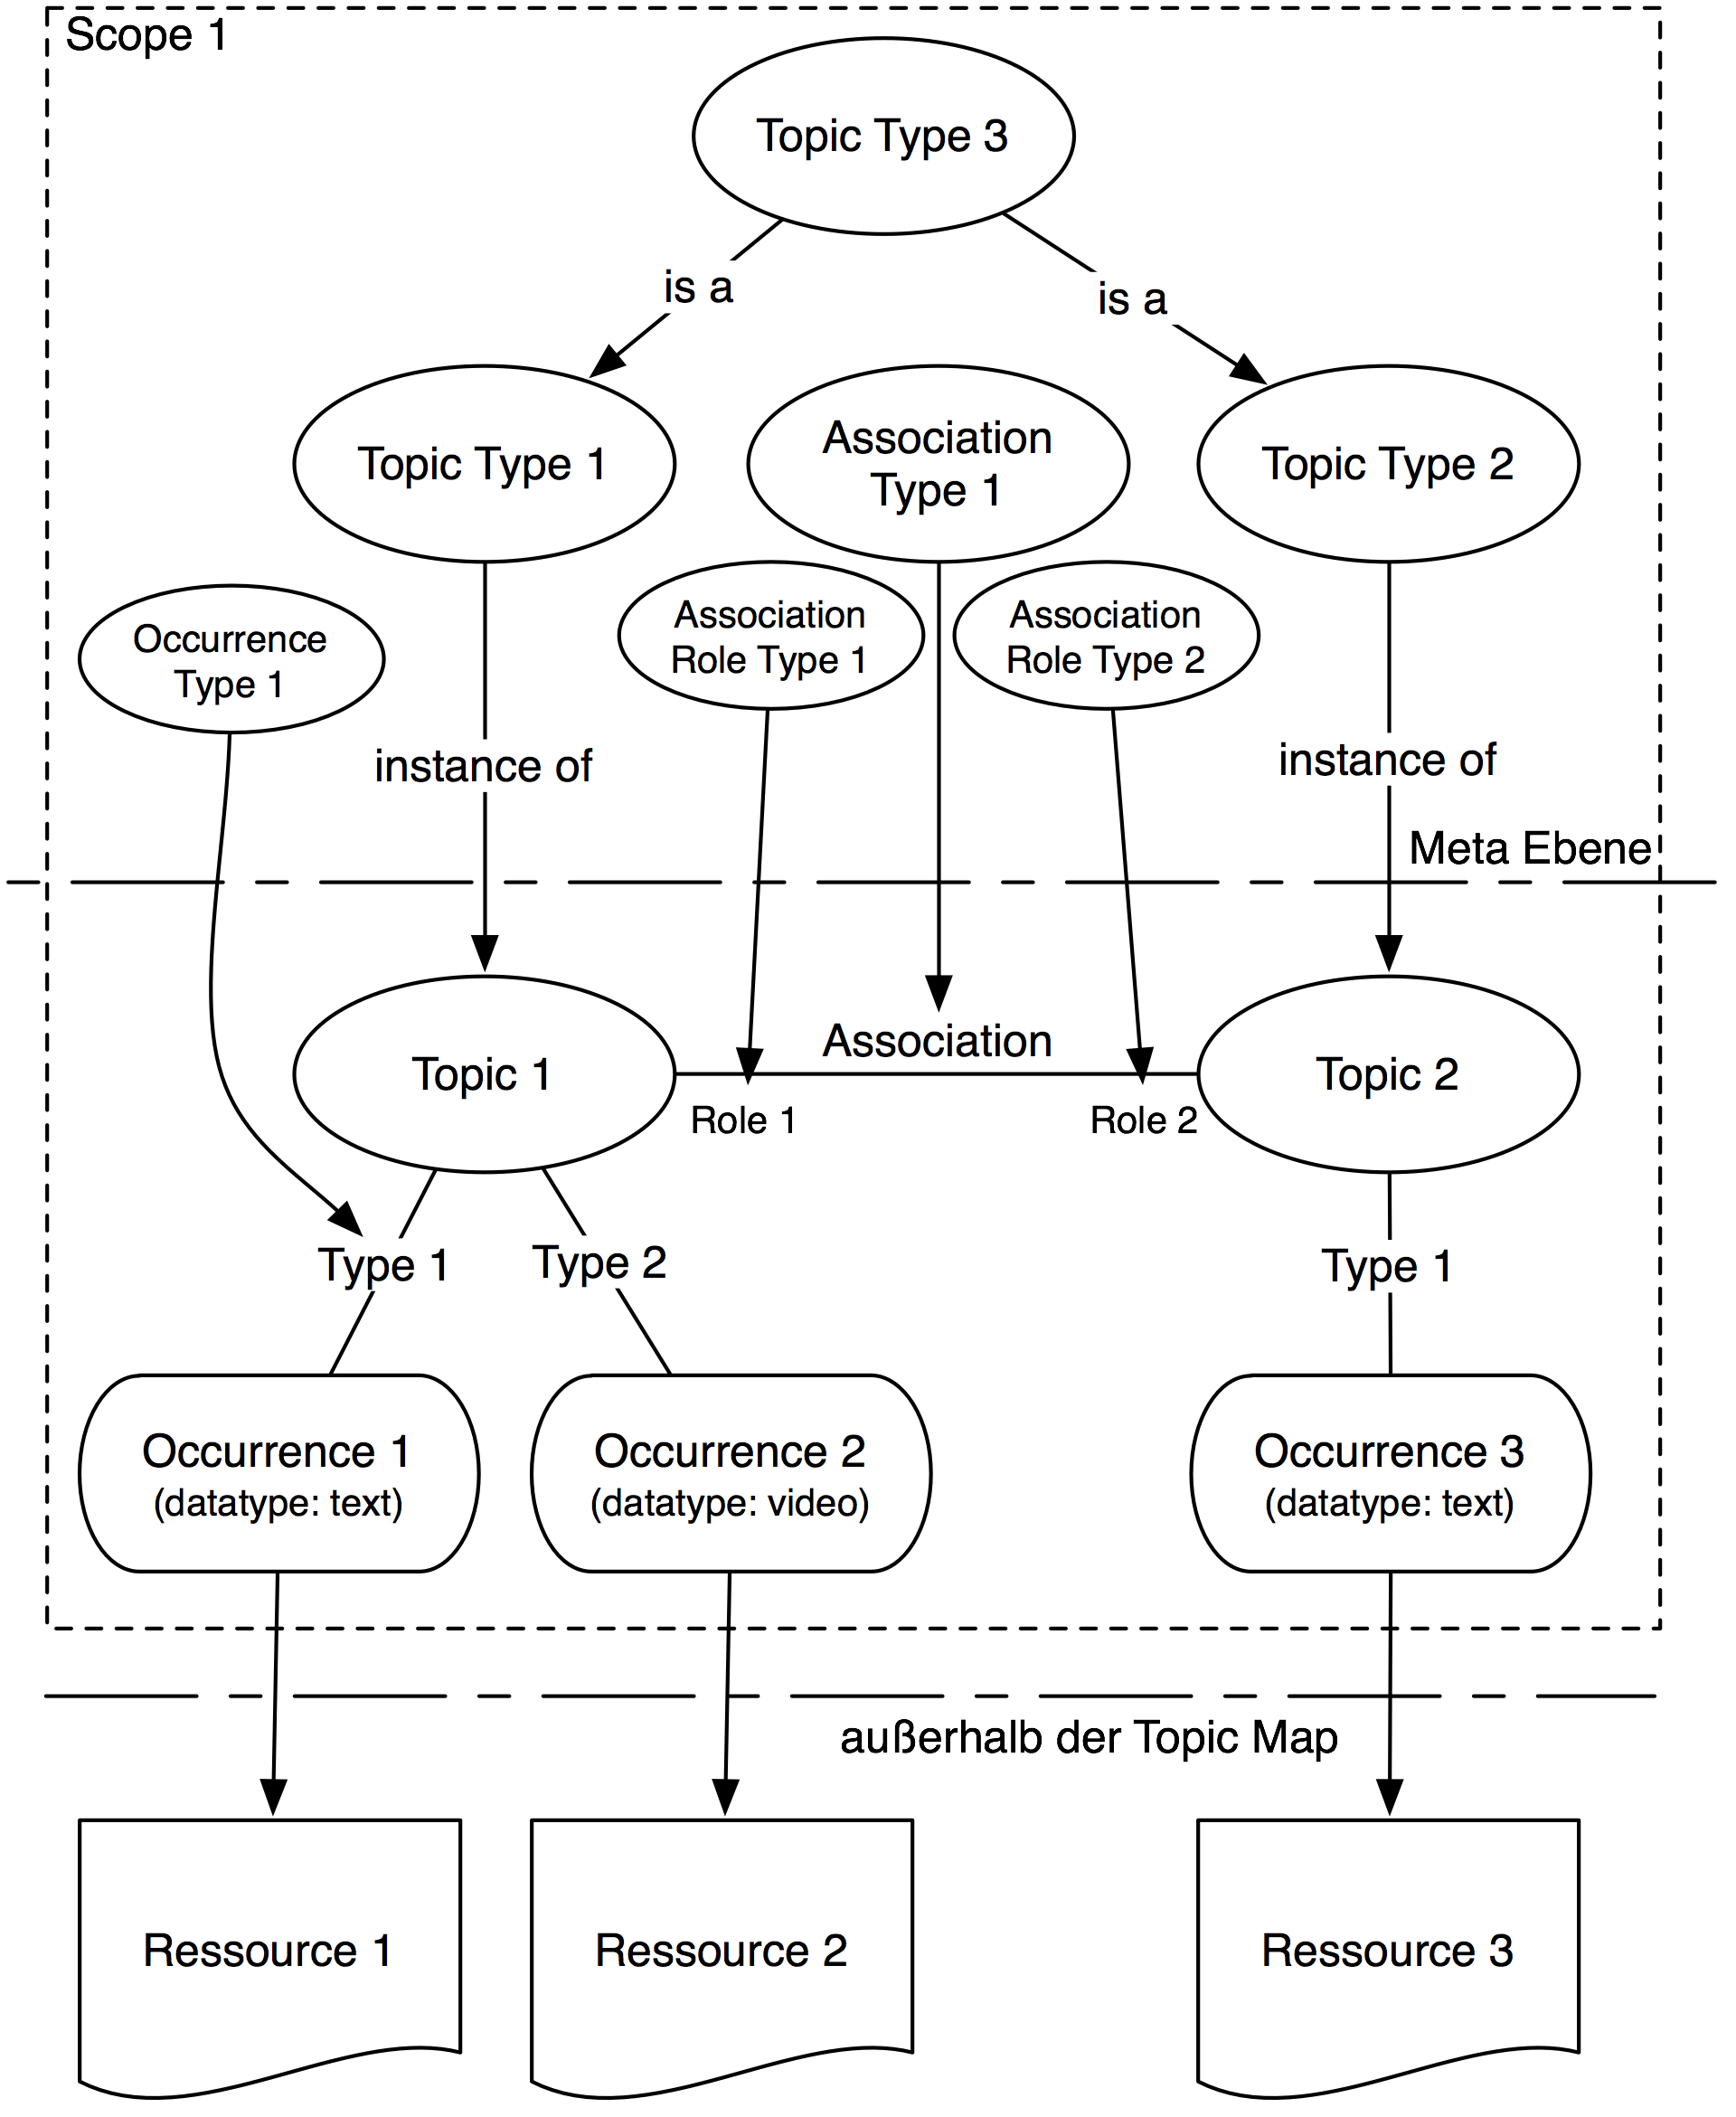
\includegraphics[width=10cm]{img/Persistenz/TMFull.png}
	\caption{Umfassende Darstellung der Elemente einer Topic Map}
	\label{fig:img_Persistenz_TMFull}
\end{figure}

\subsection{Topics, Subjects, Topic Names und Variants} % (fold)
\label{sub:topics_subjects_topic_names_und_variants}

Wie oben bereits beschrieben, repräsentiert ein Topic ein Phänomen der realen Welt in einer Topic Map. Dieses Phänomen der realen Welt, das durch das Topic repräsentiert wird, wird als „Subject“ bezeichnet. In einer Topic Map darf es zu einem Subject nur exakt ein Topic geben, umgekehrt kann ein Topic auch nicht mehrere Subjects repräsentieren, die Zuordnung zwischen Subject und Topic ist also eineindeutig (bijektiv). Im Topic wird dazu exakt ein „Subject Identifier“ registriert, der auf eine Informationsressource verweist, die das Subject für Menschen eindeutig identifizierbar macht (diese Ressource wird als „Subject Indicator“ bezeichnet). Zusätzlich kann ein „Subject Locator“ angegeben werden, der auf das tatsächlich in der realen Welt vorhandene Subject verweist. In Abgrenzung dazu kann es bei der anderen Brücke zwischen realer Welt und Topic Map, den Occurrences, für jeder Topic beliebig viele Zuordnungen geben. Eine Occurrence referenziert auch auf die reale Welt, zeigt aber dort nicht auf das Subject selbst, sondern auf ein dieses Subject beschreibendes Objekt in der realen Welt. Beispielhaft ist dazu in Abbildung \ref{fig:img_Persistenz_SubjectVsOccurrence} dieser Zusammenhang anhand des Topics „Tasse“ dargestellt. Ein anderes Beispiel ist ein Topic „London“, das als Subject die reale Stadt London repräsentiert und dem eine Occurrence zugeordnet werden könnte, die auf eine Landkarte (als in der Realität vorhandene Beschreibung der realen Stadt London) referenziert.

\begin{figure}[htbp]
	\centering
		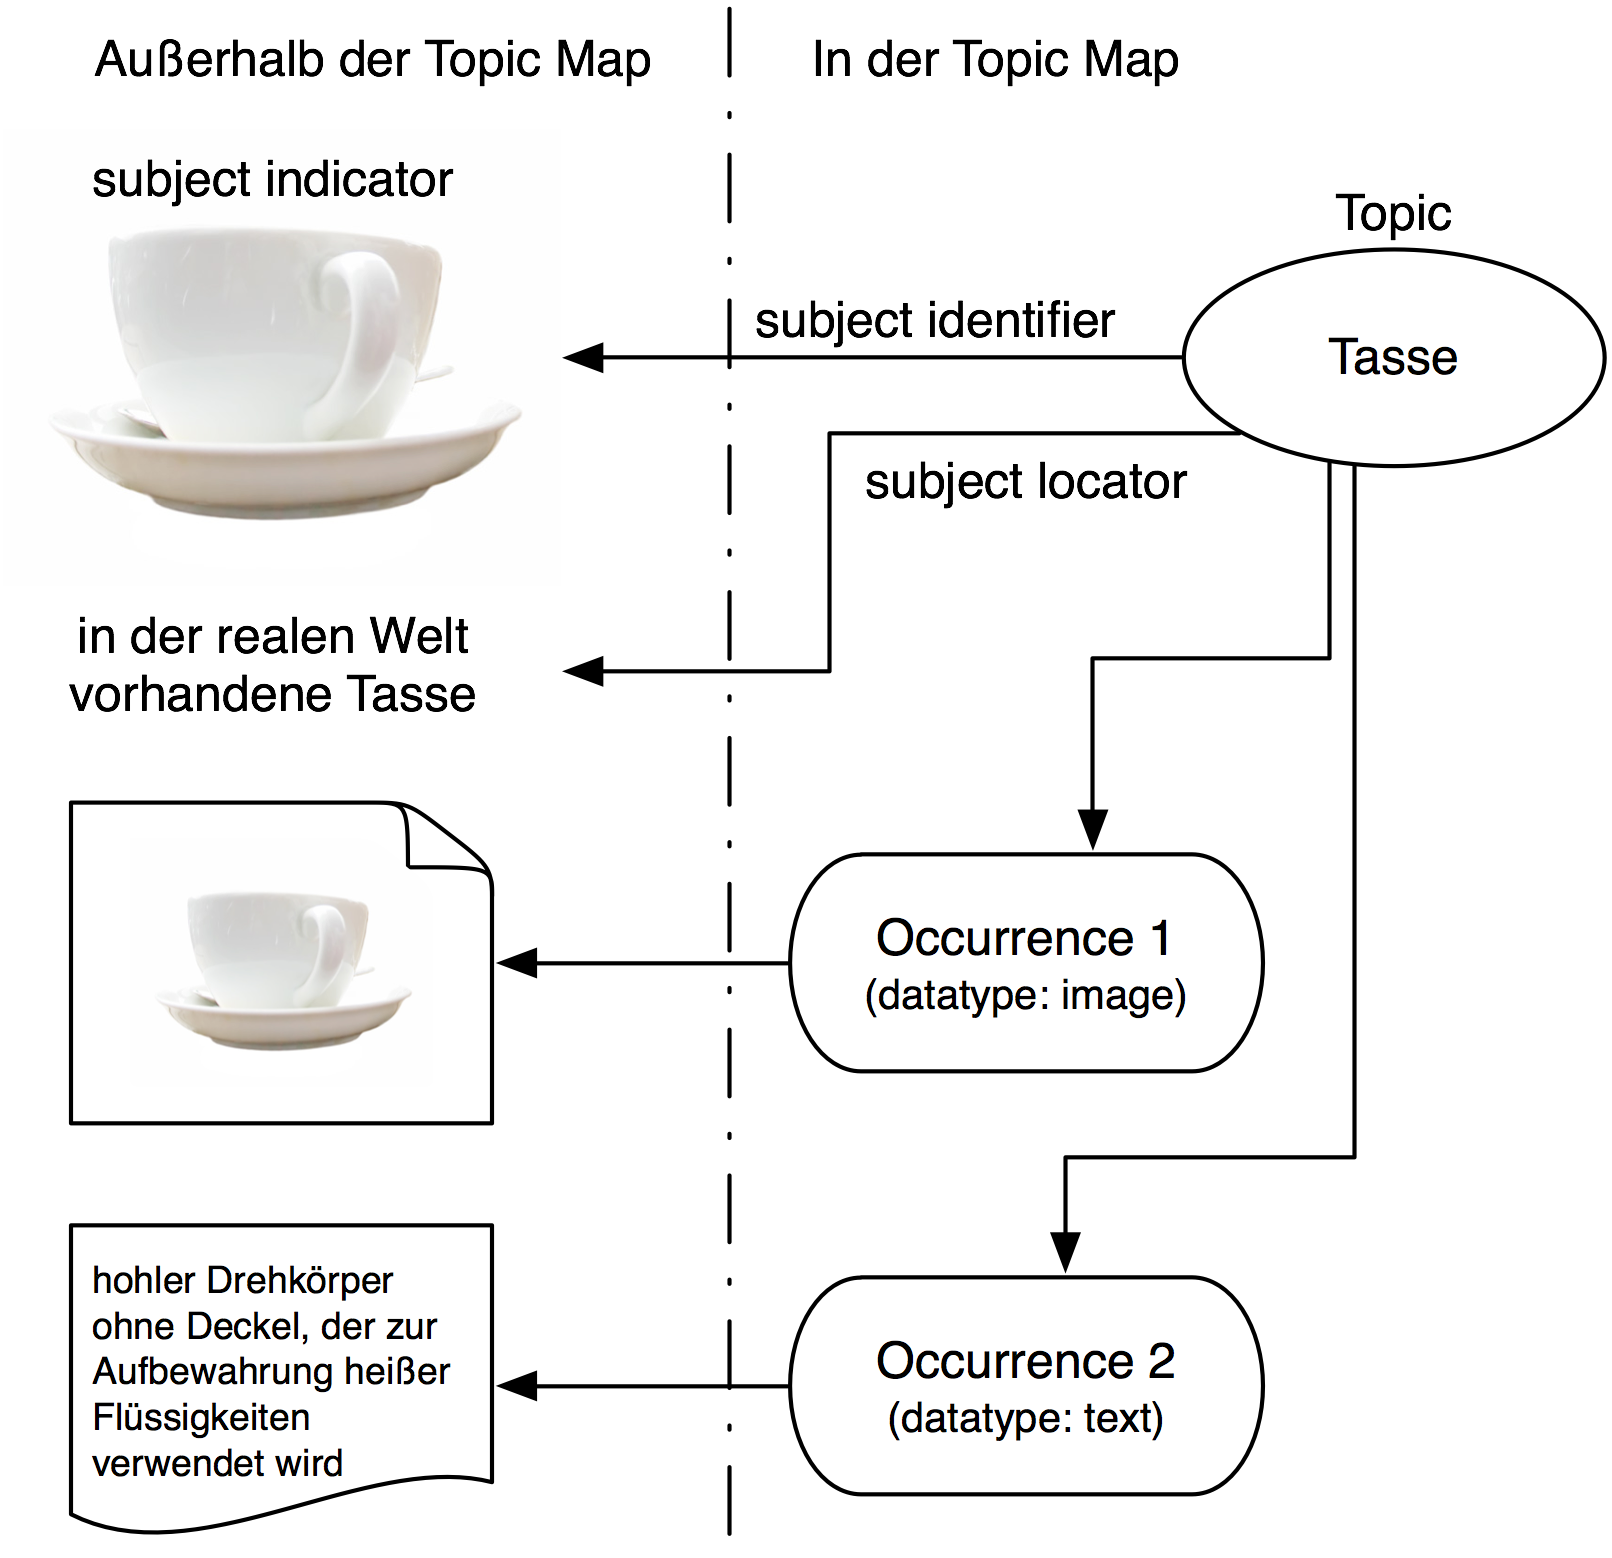
\includegraphics[width=10cm]{img/Persistenz/SubjectVsOccurrence.png}
	\caption{Abgrenzung zwischen Subject und Occurrence in Topic Maps}
	\label{fig:img_Persistenz_SubjectVsOccurrence}
\end{figure}

Bislang wurde vereinfacht ein Topic immer mit einem direkt zugeordneten Namen dargestellt. In einer Topic Map besitzt ein Topic jedoch keinen eindeutigen Namen. Es wird vielmehr durch seinen Subject Identifier eindeutig gekennzeichnet. Dieser ist jedoch nicht unbedingt für Menschen les- und/oder interpretierbar -- der Subject Identifier hat das Ziel, ein Subject für die Verarbeitung durch Software eindeutig zuordenbar zu machen. Für die Bezeichnung eines Topics in einer für Menschen interpretierbaren Form ist die Verwendung von „Topic Names“ vorgesehen (siehe Abbildung \ref{fig:img_Persistenz_TopicNaming}). Topic Names werden immer textuell angegeben und beschreiben das Subject, das durch das betreffende Topic referenziert wird. Durch einen Topic Name soll das Subject für Menschen erkennbar sein, wobei die Zuordnung nicht notwendigerweise eindeutig sein muss (Beispiel: der Topic Name „Jaguar“ kann ein Fahrzeug oder eine Großkatze bezeichnen und ist dementsprechend ein zulässiger Name für zwei unterschiedliche Topics). Einem Topic können beliebig viele Topic Names zugewiesen werden -- es ist so zum Beispiel möglich, eine mehrsprachige Topic Map zu realisieren, in der zu jedem Topic Topic Names in unterschiedlichen Sprachen angegeben werden. 

\begin{figure}[htbp]
	\centering
		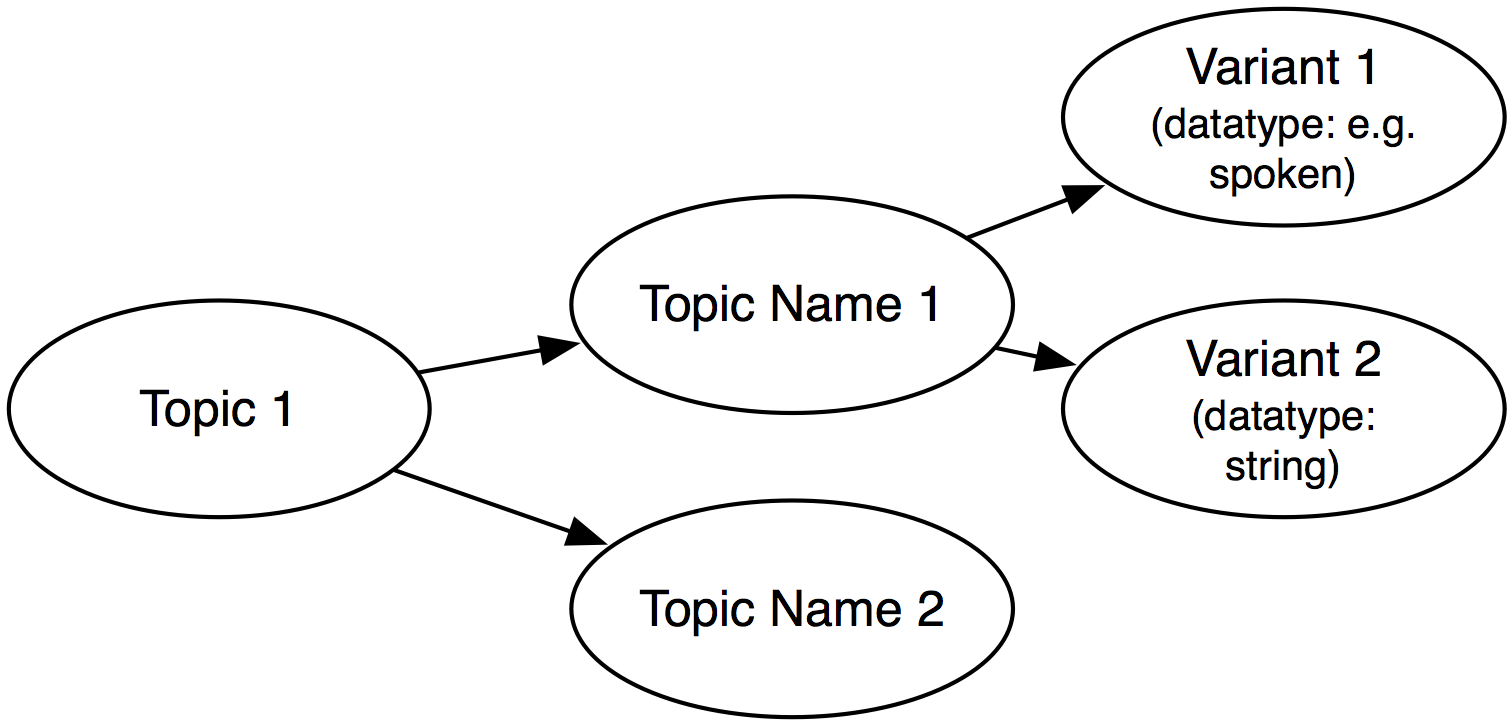
\includegraphics[width=10cm]{img/Persistenz/TopicNaming.png}
	\caption{Benennung von Topics}
	\label{fig:img_Persistenz_TopicNaming}
\end{figure}

Als weitere Detaillierungsstufe können zu jedem Topic Name „Variants“ angegeben werden. Wie durch den Namen angedeutet, handelt es sich dabei um Varianten eines Topic Names, die in bestimmten Zusammenhängen oder für gewisse Anwendungszwecke besser geeignet sein können als der eigentlich Topic Name. Ein Beispiel für eine mögliche Variante ist die Angabe einer gesprochenen Version des Topic Names. Ein weiteres Anwendungsgebiet für Varianten ist die im Standard explizit vorgesehene Angabe eines „Sort Name“ \citep[][S. 18]{TMDM08}, der es erlauben soll, Topic Maps in eine durch diesen Namen vorgegebene Ordnung bringen zu können. Varianten werden durch die Angabe eines dezidiert dafür gewidmeten Topics in deren Scope (siehe Abschnitt \ref{sub:scopes}) als Sort Names gekennzeichnet.

% subsection topics_subjects_topic_names_und_variants (end)

\subsection{Associations und Roles} % (fold)
\label{sub:associations_und_roles}

“Associations“ stellen Verbindungen zwischen den einzelnen Topics einer Topic Map her. Associations haben beliebig viele Endpunkte, mindestens jedoch einen (sind also nicht von vorneherein immer binär sondern können auch unär sein oder mehr als zwei Topics verknüpfen). Eine Associations enthält wie ein Topic nicht unmittelbar einen für Menschen lesbaren Namen. Diese wird durch ein Topic festgelegt, das die Kategorie festlegt, der die Association zuzuordnen sind (siehe Abschnitt \ref{sub:metamodellierung_in_topic_maps}). Diesem Topic kann wiederum mindestens ein Topic Name zugeordnet werden, welcher letzendlich die Benennung der Association festlegt.

Associations werden jedoch nicht direkt mit Topics verknüpft. Um ausdrucksstärkere Verknüpfungen realisieren zu können, agieren „Roles“ als Verknüpfung zwischen Association und den betreffenden Topics. Roles legen die „Rolle“ -- also die Bedeutung -- eines Topics in exakt der betrachteten Association fest. Diese Bedeutung kann generisch sein und zum Beispiel dazu verwendet werden, die per se ungerichteten Associations unabhängig von ihrer konkreten Bedeutung mit einer Richtung zu versehen (zum Beispiel durch die Zuordnung von Roles „Anfang“ und „Ende“) aber auch um die Beziehung semantisch anzureichern (zum Beispiel durch die Zuordnung von Roles „Veranwortlicher“, „Ausführender“ und „Prozessschritt“ in einer Association „durchzuführen“). Die Anzahl der in einer Association referenzierten Roles gibt damit auch die Kardinalität der Association (also die Anzahl ihrer Endpunkte) an. Aus den konkreten Roles wird dann auf die Topics verwiesen, die diese Roles einnehmen bzw. „spielen“ (tatsächlich heißt die betreffende Eigenschaft einer Role „player“). Genau wie Associations werden Roles nicht direkt benannts sondern über ein Topic, das ihre Kategorie bestimmt, mit einer Benennung versehen (Detail wiederum in Abschnitt \ref{sub:metamodellierung_in_topic_maps}).

% subsection associations_und_roles (end)

\subsection{Occurrences und Datatypes} % (fold)
\label{sub:occurrences_und_datatypes}

Wie zu Beginn dieses Abschnitts bereits beschrieben und in den Erläuterungen zur Thematik der Subjects (siehe Abschnitt \ref{sub:topics_subjects_topic_names_und_variants}) angedeutet, bilden „Occurrences“ die Brücke aus der Topic Map in die reale Welt, indem sie auf Ressourcen referenzieren, die in einem beliebigen Zusammenhang mit den jeweiligen Topic stehen. Ein Topic kann beliebig viele Occurrences haben. Anders als bei Associations existieren für Occurrences keine Roles (was auch nur bedingt sinnvoll wäre, da jede Occurrence nur zu exakt einem Topic gehören kann). Die Bedeutung der Occurrence für das Topic kann wie bei Associations über die Kategorie der Occurrence festgelegt werden, die wiederum durch ein separates Topic repräsentiert wird (siehe dazu auch Abschnitt \ref{sub:metamodellierung_in_topic_maps}). Beispielsweise kann eine Occurrence zur Kategorie „Karte“ gehören und so angeben, dass die so klassifizierte Occurrence zum Topic „London“ auf eine Karte des Stadtgebiets verweist.

Zusätzlich zu der Kategorie wird in einer Occurrence auch der Datentyp der Information angegeben, in dem die referenzierte Information vorliegt. Dabei können beliebige URI (Uniform Resource Identifiers\footnote{wie in RFC 3986 definiert und unter http://www.ietf.org/rfc/rfc3986.txt abzurufen}) verwendet werden. Da URIs beliebigen Inhalt haben können, wäre es in obigen Beispiel möglich durch den Datentyp einer Occurrence festzulegen, ob es sich bei der Karte um eine Rastergrafik oder eine Vektorgrafik handelt und so Information über deren möglich Einsatzgebiete zu einzubetten.

% subsection occurrences_und_datatypes (end)

\subsection{Metamodellierung in Topic Maps} % (fold)
\label{sub:metamodellierung_in_topic_maps}

Wie oben bereits mehrmals angedeutet kann in einer Topic Map neben den eigentlichen zu repräsentierenden Informationen (Topics, Associations, Roles und Occurrences) auch Information über die Topic Map selbst eingebettet werden (neben dem Model also auch das Meta-Modell abgebildet werden kann). Die Information umfasst Angaben über die in der jeweiligen Topic Map existierenen Kategorien von Topics, Topic Names, Associations, Roles und Occurrences. Hinsichlich der Repräsentation dieser Information sind zwei Ansätze zu unterscheiden, von denen der erste bei Kategorieangaben von Topics zum Einsatz kommt, der andere bei Kategorieangaben jeder anderen Art von Information. Allen Kategorien ist gemein, dass sie selbst wiederum als Topics repräsentiert werden und auch als solche verwendet werden können. Es ist also möglich, zu einem Topic, das als Kategorie verwendet wird, selbst wiederum eine Kategorie anzugeben, wodurch die Einführung beliebig vieler Meta-Ebenen möglich ist. Außerdem können als Kategorien verwendete Topics ebenfalls wieder mit Associations verknüpft und mit Occurrences versehen werden. Hinsichtlich der Nomenklatur ist noch darauf hinzuweisen, dass Kategorien im Allgemeinen als „Types“ bezeichnet werden, man also von „Topic Types“, „Topic Name Types“, „Association Types“, „Role Types“ und „Occurrence Types“ spricht.

\subsubsection{Topic Types}

Topic Types werden in einer Topic Map durch ein spezielle, im Standard festgelegte Association definiert. Soll einem Topic ein Type zugewiesen werden, muss eine Association der Kategorie „type-instance“ eingefügt werden, bei der das Topic selbst die Role „instance“ einnimmt und dem Topic, das die Kategorie repräsentiert, die Role „type“ zugewiesen wird. Diese Beziehung entspricht einer Konkretisierung eine (abstakten) Kategorie oder Klasse von Topics auf eine bestimmte Instanz, die die Merkmale dieser Klasse trägt. In Abbildung \ref{fig:img_Persistenz_MetaModelExample} besteht eine type-instance-Beziehung (dort als „instance-of“ bezeichnet) zwischen der Kategorie „VW Golf“ und der konkreten Instanz „SR-174 AU“ (also einem Topic, bei dem das amtliche Kennzeichen als Topic Name verwendet wurde). „VW Golf“ fungiert hier also als Topic Type, wobei es selbst ein Topic ist, das sich durch nichts als die eingenomme „type“-Rolle von einem anderen Topic unterscheidet und dementsprechend behandelt werden kann.

Einem Topic können beliebig viele Topic Types zugewiesen werden, indem es in mehr als einer Association die Role „instance“ einnimmt. Es wird so als mehreren Kategorien zugehörig gekennzeichnet. Umgekehrt kann ein Topic Type mehr als einem Topic zugewiesen werden, indem das betreffende den Topic Type repräsentierende Topic die Role „type“ mehrfach einnimmt.

\begin{figure}[htbp]
	\centering
		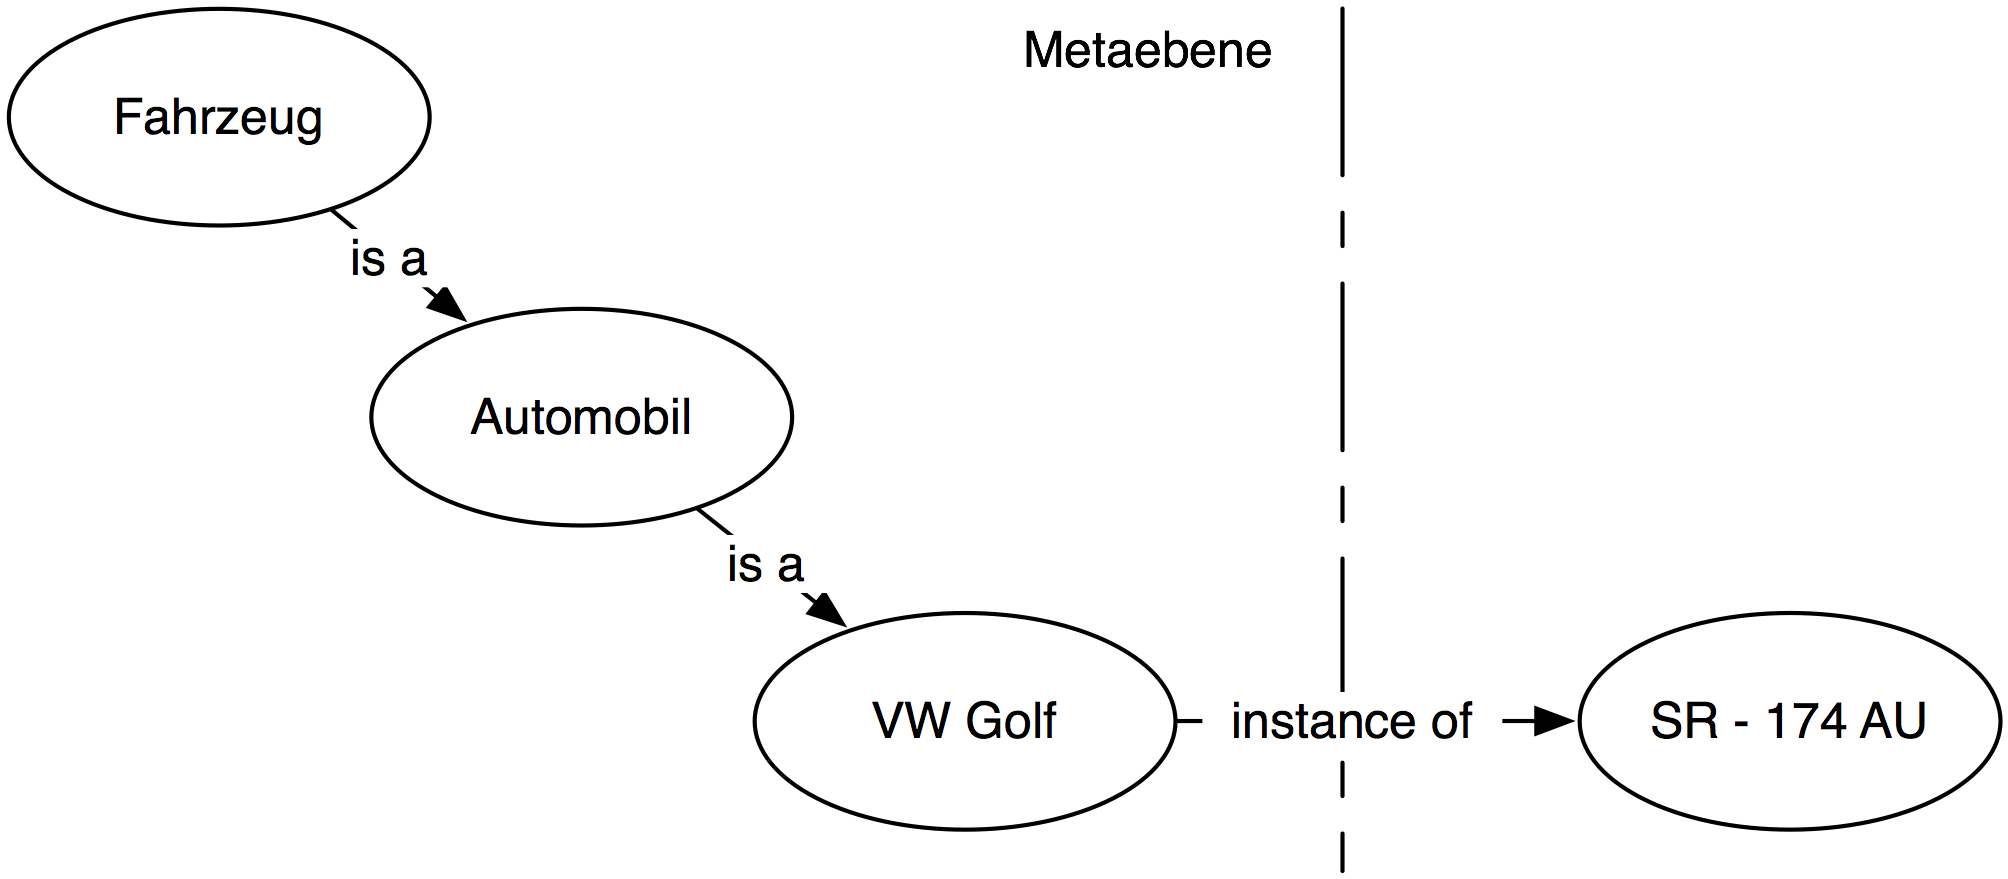
\includegraphics[width=10cm]{img/Persistenz/MetaModelExample.png}
	\caption{Beziehungen in der Metamodellbildung in Topic Maps}
	\label{fig:img_Persistenz_MetaModelExample}
\end{figure}

Auch ist es möglich, Hierarchien von Types zu bilden, in dem einem Topic, das als Topic Type fungiert, selbst wieder ein Topic Type zugewiesen wird. Dieses Konstrukt ist jedoch mit Vorsicht zu gebrauchen, da zur Abbildung der Struktur einer Domäne ein semantisch ähnliches, bei näherer Betrachtung aber eine unterschiedliche Bedeutung tragendes Konstrukt zum Einsatz kommt. Grundsätzlich muss unterschieden werden, ob ein Topic eine konkrete Instanz eines anderen ist oder lediglich eine Spezialisierung darstellt. Im ersteren Fall kommt eine „type-instance“ zum Einsatz, das übergeordnete Topic befindet sich semantisch auf eine anderen, abstrakteren Ebene und stellt eine Kategorie (also einen Topic Type) dar. Im Falle einer Spezialisierung kommt eine „supertype-subtype“-Association zum Einsatz, deren Rollen „supertype“ vom übergeordneten, allgemeineren bzw. „subtype“ vom untergeordneten, spezielleren Topic eingenommen wird. Hier befinden sich beide Topics semantisch auf einer Ebene, keines ist abstrakter als das andere. Der Unterschied liegt vielmehr in der mehr oder weniger konkreten Festlegung der durch die Topics repräsentierten Subjects. So ist wie in Abbildung \ref{fig:img_Persistenz_MetaModelExample} dargestellt das Topic „VW Golf“ ein Subtype des Topics „Automobil“ welches wiederum ein Subtype des Topics „Fahrzeug“ ist. Hier ist erkennbar, dass „Automobil“ insofern eine Spezialisierung von „Fahrzeug“ ist, als dass es im Allgemeinen motorisiert ist und vier Räder besitzt. „VW Golf“ ist wiederum eine Spezialisierung von Fahrzeug, die hinsichtlich der Form der Karosserie, der Anzahl der Türen und anderen Merkmalen mehr spezialisiert. Zwischen keinem der Topics findet jedoch eine Konkretisierung in dem Sinne statt, als dass auf der untergeordneten Seite von einem konkreten, real existierenden Fahrzeug die Rede wäre -- dazu ist die „type-instance“-Beziehung zu verwenden. Die „subtype-supertype“-Beziehung ist transitiv, d.h. dass ein „VW Golf“ nicht nur ein „Automobil“ ist, sondern auch ein „Fahrzeug“. Für „type-instance“-Beziehungen ist diese Eigenschaft nicht gegeben. 

\subsubsection{Andere Types}

Bei allen anderen Types (konkret also Topic Name Types, Association Types, Role Types und Occurrence Types) wird die Kategorie nicht durch eine separate Association abgebildet sondern durch eine im jeweiligen Informationselement enthaltene Referenz auf ein Topic, das als Type fungiert. Die Darstellung der Kategorie-Information ist damit nicht so explizit wie bei Topic Types, wo sich direkt in der Repräsentation der eigentlichen Nutzinformation niederschlägt. Auch semantisch ist sind die hier behandelten Types gegenüber Topic Types insofern eingeschränkt, als das jedem Element exakt ein Type zugeordnet sein muss (der Type kann also nicht leer sein, auch können nicht mehrere Types zugeordnet werden). Wie oben bereits erwähnt sind Topic Types hier flexibler, einem Topic können beliebig viele oder auch keine Topic Types zugeordnet werden. Dies ist aber nur vordergründig eine Einschränkung. Topics dürfen wie oben beschrieben für jedes Subjekt nur einmal existieren. Hat aber ein Subject und damit ein Topic in unterschiedlichen Domänen unterschiedliche Bedeutungen, muss dies über mehrere Topic Types (in Verbindung mit Scopes, siehe Abschnitt \ref{sub:scopes}) abgebildet werden. Alle anderen Informationskategorien in der Topic Map unterliegen nicht dieser Eineindeutigkeitsregel und können bzw. müssen, sollten sie unterschiedlichen Kategorien zuzuordnen sein, auch mehrfach vorhanden sein. Eine Assoziation, die einen anderen Namen trägt (also einer anderen Kategorie angehört) ist beispielsweise nicht identisch mit der ursprünglichen Assoziation, deren Name ebenfalls bereits durch die Zuordnung zu einer Kategorie festgelegt wurde. 

\subsubsection{Modellieren von Einschränkungen}

Der Topic Map Standard erlaubt zwar die Angabe von Metamodellelementen (Types), ermöglicht es aber nicht Regeln anzugeben, anhand derer der semantisch korrekte Aufbau einer Topic Map geprüft werden. Ed ist beispielsweise möglich, einen Association-Type „hat Mitglieder“ zu definieren, der mittels den Roles „Organisationseinheit“ und „Mitarbeiter“ die Zuordnung von Mitarbeitern zu den Organisationseinheiten eines Unternehmens zuzuordnen. Es ist jedoch in der Topic Map nicht möglich zu spezifizieren, das beispielsweise mindestens drei Mitarbeiter zugeordnet werden müssen oder das es in dieser Beziehung nur eine Organisationseinheit geben darf. Weiters kann nicht spezifiziert werden, durch Topics welchen Types die jeweiligen Roles eingenommen werden dürfen -- beispielsweise ist eine Zuordnung von Produktionsmitteln in der Role „Mitarbeiter“ zulässig bzw. kann sie nicht als unzulässig gekennzeichnet werden.

Ist eine derartige semantische Einschränkung bei der Topic Map Erstellung und die Einführung verbindlicher Strukturvorgaben notwendig, so muss dies außerhalb der Topic Map oder durch externe Interpretation spezifischer Topic Map Elemente geschehen. In ersterem Fall kann die noch nicht in finalem Zustand vorliegende TMCL (Topic Map Constraint Language, \citep{TMCL08}), eine Regelsprache zur Einschränkung der Repräsentationsmöglichkeiten in einer Topic Map, verwendet werden. Im zweiten Fall können die Metamodell-Elemente (also alle Topics, die als Types verwendet werden) durch zusätzliche Associations verknüpft werden, die semantisch so interpretiert werden, dass sie eine zulässige Kombination von Topics der jeweiligen Kategorie anzeigen.

% subsection metamodellierung_in_topic_maps (end)

\subsection{Statements und Scopes} % (fold)
\label{sub:scopes}

Topic Maps bieten die Möglichkeit, Gültigkeitsbereiche für die in ihnen abgebildeten Informationen zu spezifizieren. Ein Gültigkeitsbereich definiert, in welchem Kontext eine Information gültig ist. Außerhalb dieses Kontext kann über die Gültigkeit keine Aussage getroffen werden. Der Gültigkeitsbereich wird als „Scope“ bezeichnet. Ein Scope kann für jedes „Statement“ in der Topic Map gesetzt werden. Statements sind alle „Aussagen“ über Topics, die in der Topic Map abgebildet werden, nicht aber Topics selbst. Als Statement werden Topic Names, Associations und Occurrences betrachtet. Roles und Variants besitzen keinen Scope, da sie keine direkte Aussage über Topics treffen, sondern nur im Zusammenhang mit Associations bzw. Topic Names existieren, deren Scope sich quasi auf sie vererbt.

Ein Scope für ein Statement wird durch die Angabe eines oder mehrerer Topics festgelegt. Wird kein Topic angegeben, so gilt der „unconstrainted scope“, das Statement ist unbeschränkt gültig. Topics zur Abbildung von Scopes können explizit angelegt werden (z.B. Topics „Deutsch“ und „Englisch“, die Sprach-Scopes ermöglichen, Topics „Tierwelt“ und „Transportwesen“ zur Domänenabgrenzung -- siehe Abbildung \ref{fig:img_Persistenz_Scope}), es ist jedoch grundsätzlich auch möglich, die Gesamtheit der Topics einer Domäne zur Definition eines betreffenden Scopes heranzuziehen (also alle in der Topic Map vorhandenen Topics, die Tiere repräsentieren, als Scope zu verwenden, um den Gültigkeitsbereich „Tierwelt“ abzubilden). Obwohl der Topic Map Standard hier explizit offen bleibt, erscheint jedoch erstere Variante hinsichtlich der Verwaltbarkeit aber auch der semantischen Vollständigkeit wegen als ratsamer (das Konzept „Tierwelt“ käme ansonsten z.B. nicht notwendigerweise vor, sondern wäre nur implizit vorhanden, was eine Auswertung schwierig macht).

\begin{figure}[htbp]
	\centering
		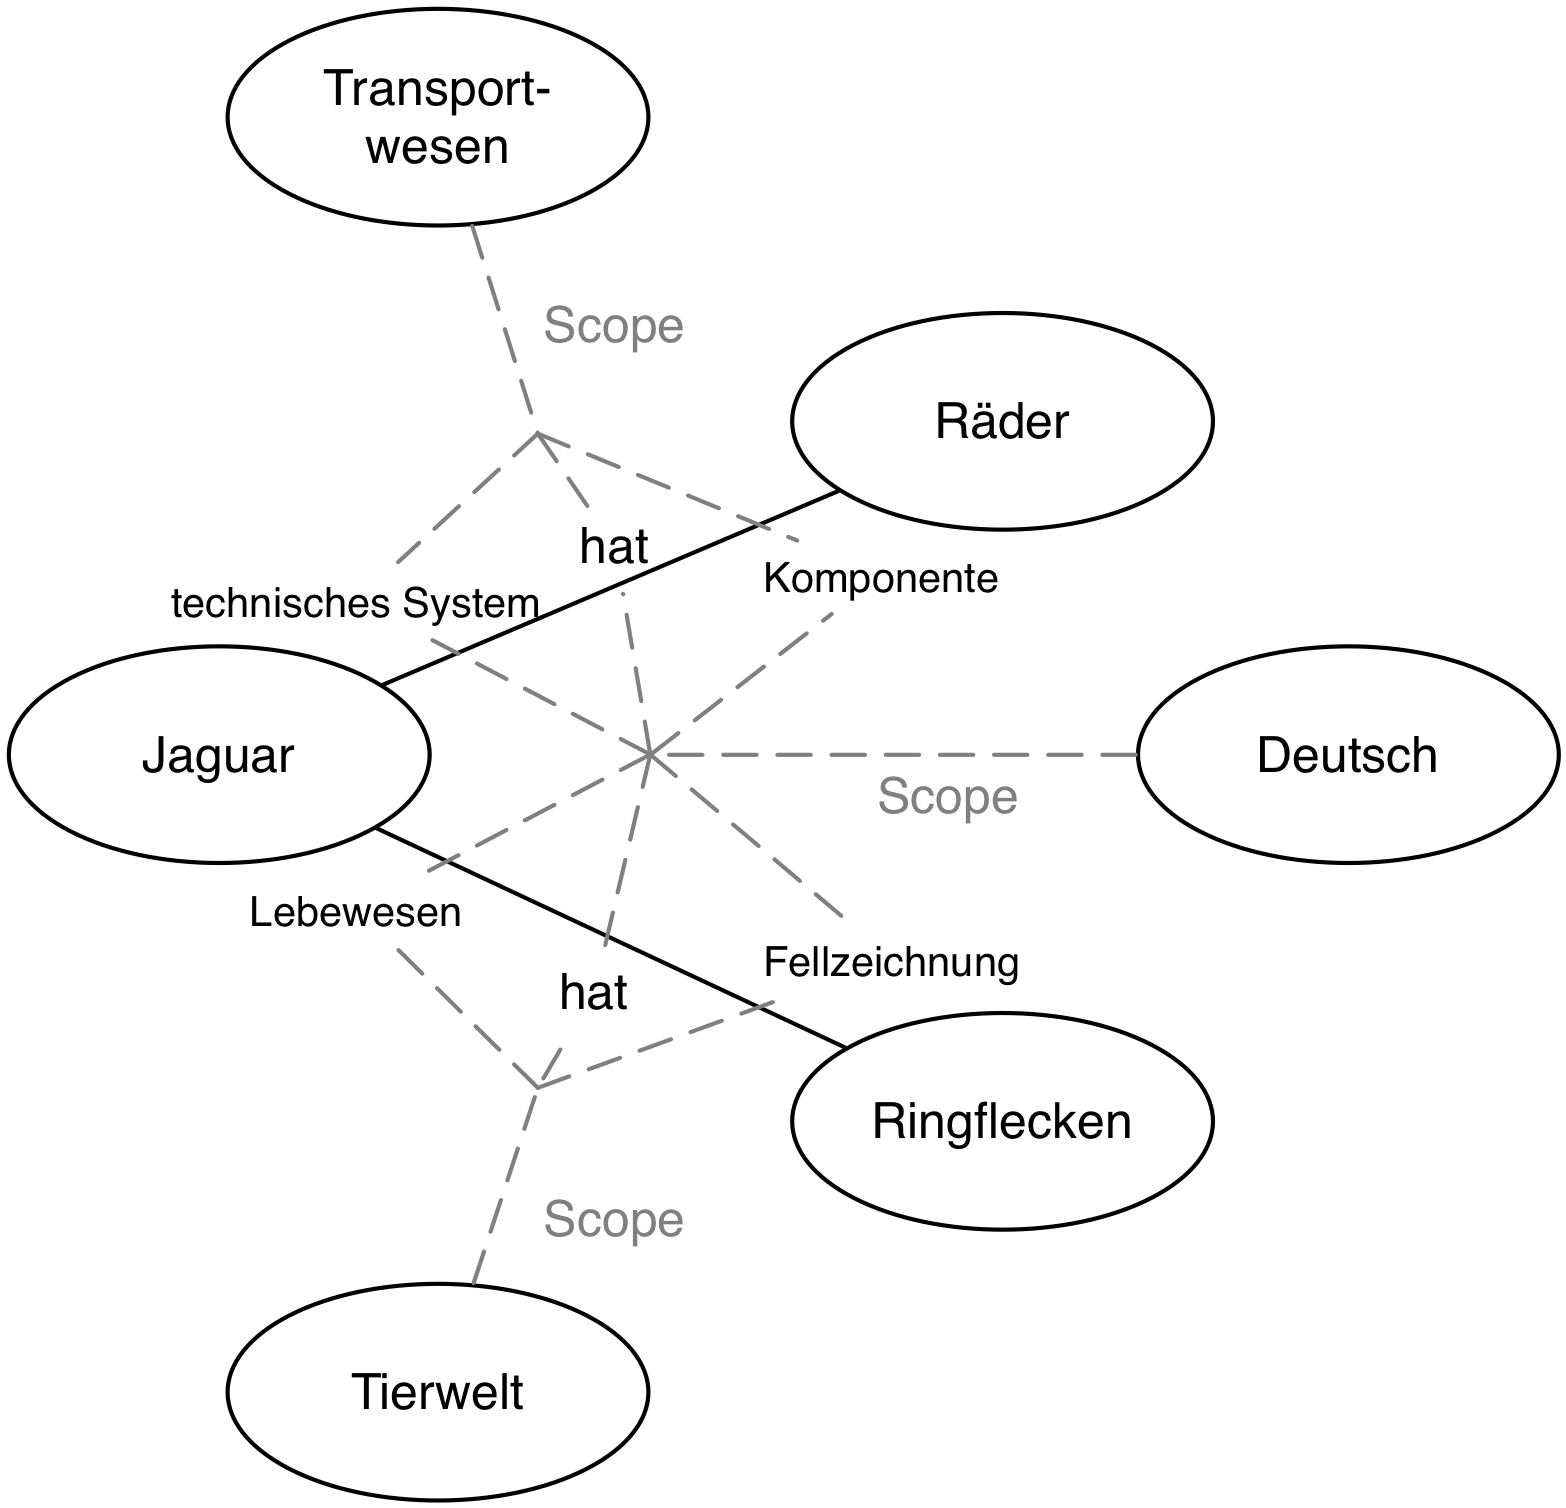
\includegraphics[height=3in]{img/Persistenz/Scope.png}
	\caption{Abbildung von Gültigkeitsbereichen durch Scopes}
	\label{fig:img_Persistenz_Scope}
\end{figure}


Wird mehr als ein Topic angegeben, so bilden alle Topics gemeinsam den Kontext, indem das Statement gültig ist. Bei der Auswertung des Gültigkeitsbereichs müssen also alle angegebenen Topics zutreffen, damit ein Statement gültig ist. Ein Statement dessen Scope die Topics „Tierwelt“ und „Deutsch“ enthält, ist also nur gültig, wenn beide Topics zutreffen (also z.B. zur Filterung ausgewählt wurden). Die gültigen Statements sind also die Schnittmenge jener der Statements, die im Scope „Tierwelt“ und im Scope „Deutsch“ gültig sind (siehe Abbildung \ref{fig:img_Persistenz_Scope}). Die Angabe eines Scopes zu einem Statement, das in beiden Scopes (unabhängig voneinander gesehen) gültig sein soll, ist nicht direkt möglich. In diesem Fall muss das Statement zweimal jeweils unter Angabe eines der beiden Scopes eingefügt werden.

Für Topics selbst kann kein Scope angegeben werden. Das ist hinsichtlich des Topic Maps zugrunde liegenden Konzepts auch nicht sinnvoll, da Topics immer ein Phänomen der realen Welt, das Subject, repräsentieren, das selbst immer vorhanden ist und dessen Gültigkeit bzw. Existenz nicht von anderen Rahmenbedingungen wie anderen Subjects abhängt. Dementsprechend existiert ein Topic immer, lediglich seine Bezeichnung, die Beziehungen zu anderen Topics oder seine Occurrences können abhängig vom einem Scope unterschiedlich sein.
% subsection scopes (end)

\subsection{Reification} % (fold)
\label{sub:reification}

Wie bereits zu Beginn angeführt, können in einer Topic Map beliebige Inhalte abgebildet werden, jegliche Phänomene der realen Welt können durch Topics repräsentiert werden. Konsequenterweise können nun auch Elemente der Topic Map selbst oder sogar die Topic Map ansich durch ein Topic dargestellt werden. Eine derartige selbstbezügliche Abbildung wird als „Reification“ bezeichnet. Der Ausgangspunkt für eine Reification kann ein Statement sein oder eine Topic Map selbst. Topics können nicht verwendet werden, da ein sie repräsentierendes Topic semantisch äquivalent mit dem Ausgangspunkt wäre und damit zwei Topics vorhanden wären, die das gleiche Subject referenzieren. Nachdem die Abbildung zwischen Subject und Topic eineindeutig sein muss, ist ein derartiges Konstrukt nicht erlaubt.

In Abgrenzung zur Types (Association Types, Occurrence Types, \ldots) repräsentiert ein reifizierendes Topic nicht die Kategorie eines Elements sondern das konkrete Element selbst. Es ist so möglich, einem konkreten Element wie einer Association zusätzliche Information hinzuzufügen (etwa eine Occurrence) oder auch eine bestehende Topic Map als Ganzes zu kapseln und durch das sie reifizierende Topic Bezug zu nehmen. 

% subsubsection reification (end)

\subsection{Merging} % (fold)
\label{ssub:merging}

Unter „Merging“ versteht man die Vereinigung zweier voneinander getrennter Topic Maps zu einer gemeinsamen Map. Dabei ist vor allem die Eineindeutigkeitsregel zu beachten, für ein Subject darf also in der resultierenden Topic Map nur ein Topic existieren. Strukturell nicht kritisch, jedoch die Verwendbarkeit einschränkend sind mehrfach auftretende semantisch identische Statements. Soweit möglich, sollten auch diese Duplikate im Merging-Prozess entfernt werden.

Der Topic Map Standard definiert für jede Art von Element Regeln, anhand der festgestellt werden kann, ob zwei Elemente dieser Art identisch sind oder nicht. Ausgangspunkt sind immer die Topics, wobei beim Vergleich ausschließlich vom abgebildeten Subject ausgegangen werden muss. Sind die Subjects identisch, sind im Wesentlichen auch die beiden Topics identisch und können durch eine gemeinsames Topic ersetzt werden. Auf Basis der vereinigten Topic Menge werden nun die enthaltenen Statements verglichen. Damit Statements als identisch erkannt werden, müssen nicht nur ihr eigentlicher Inhalt sondern auch ihre Kategorie (Type), ihr Gültigkeitsbereich (Scope) und das/die ihnen zugeordnete(n) anderen Element(e) identisch sein. Eine Role ist also nur dann mit einer anderen Role identisch, wenn ihr Type, ihr Scope, die Association, der sie angehört und das referenzierte Topic identisch ist. Daraus folgt, das in der Merging-Reihenfolge zuerst die Topics, dann die eigenständigen Statements wie Topic Names, Associations und Occurrences und letztendlich die abgängigen Statements wie Roles und Variants behandelt werden müssen.
% subsubsection merging (end)

% section topic_maps (end)

\section{Abbildung von Modellen auf Topic Maps} % (fold)
\label{sec:abbildung_von_modellen_auf_topic_maps}

Diagrammatische Modelle \citep{Oppl05a} können direkt ohne zusätzliche Transformationen auf Topic Maps abgebildet werden. Derartige Modelle bestehen aus Knoten und Kanten, die Verwendung dieser im konkreten Anwendungskontext ist durch die Modellierungssprache festgelegt. In den folgenden Abschnitten wird nun beschrieben, wie die einzelnen Aspekte eines diagrammatischen Modells auf eine Topic Map abgebildet werden können.

\subsection{Grundlegende Abbildung} % (fold)
\label{sub:grundlegende_abbildung}
Der nahe liegendste Ansatz, um diagrammatische Modelle auf Topic Maps abzubilden, werden nun die Knoten auf Topics, die Kanten auf Associations abzubilden (siehe Abbildung \ref{fig:img_Persistenz_AssociationReification}, Variante 1). Ist in den Kanten mehr Information als die bloße Anzeige der Verbindung von zwei Knoten abgebildet (wie z.B. in \gls{UML} State Charts \citep{Rumbaugh04}, bei denen die zu einem Zustandsübergang führenden Ereignisse inkl. Bedingungen und ablaufende Aktionen in den Kanten repräsentiert werden), so kann es sinnvoll sein, auch die Kanten auf Topics abzubilden, da diesen auf dem Wege der Occurrences zusätzliche Information zugewiesen werden kann (siehe Abbildung \ref{fig:img_Persistenz_AssociationReification}, Variante 2). Associations würden in diesem Fall verwendet, um die Knoten und Kanten des Modells zu verbinden, spielen also in der Repräsentation der Information nur noch ein untergeordnete Rolle. Ein Weg, die direkte Abbildung beizubehalten (indem Knoten auf Topics und Kanten auf Associations abgebildet werden) ist, zur Repräsentation der zusätzlich in den Kanten liegenen Information die Möglichkeit der Reification zu nutzen, den Associations also Topics zuzuweisen, die genutzt werden können, um diese zusätzliche Information zu verwalten (siehe Abbildung \ref{fig:img_Persistenz_AssociationReification}, Variante 3).

\begin{figure}[htbp]
	\centering
		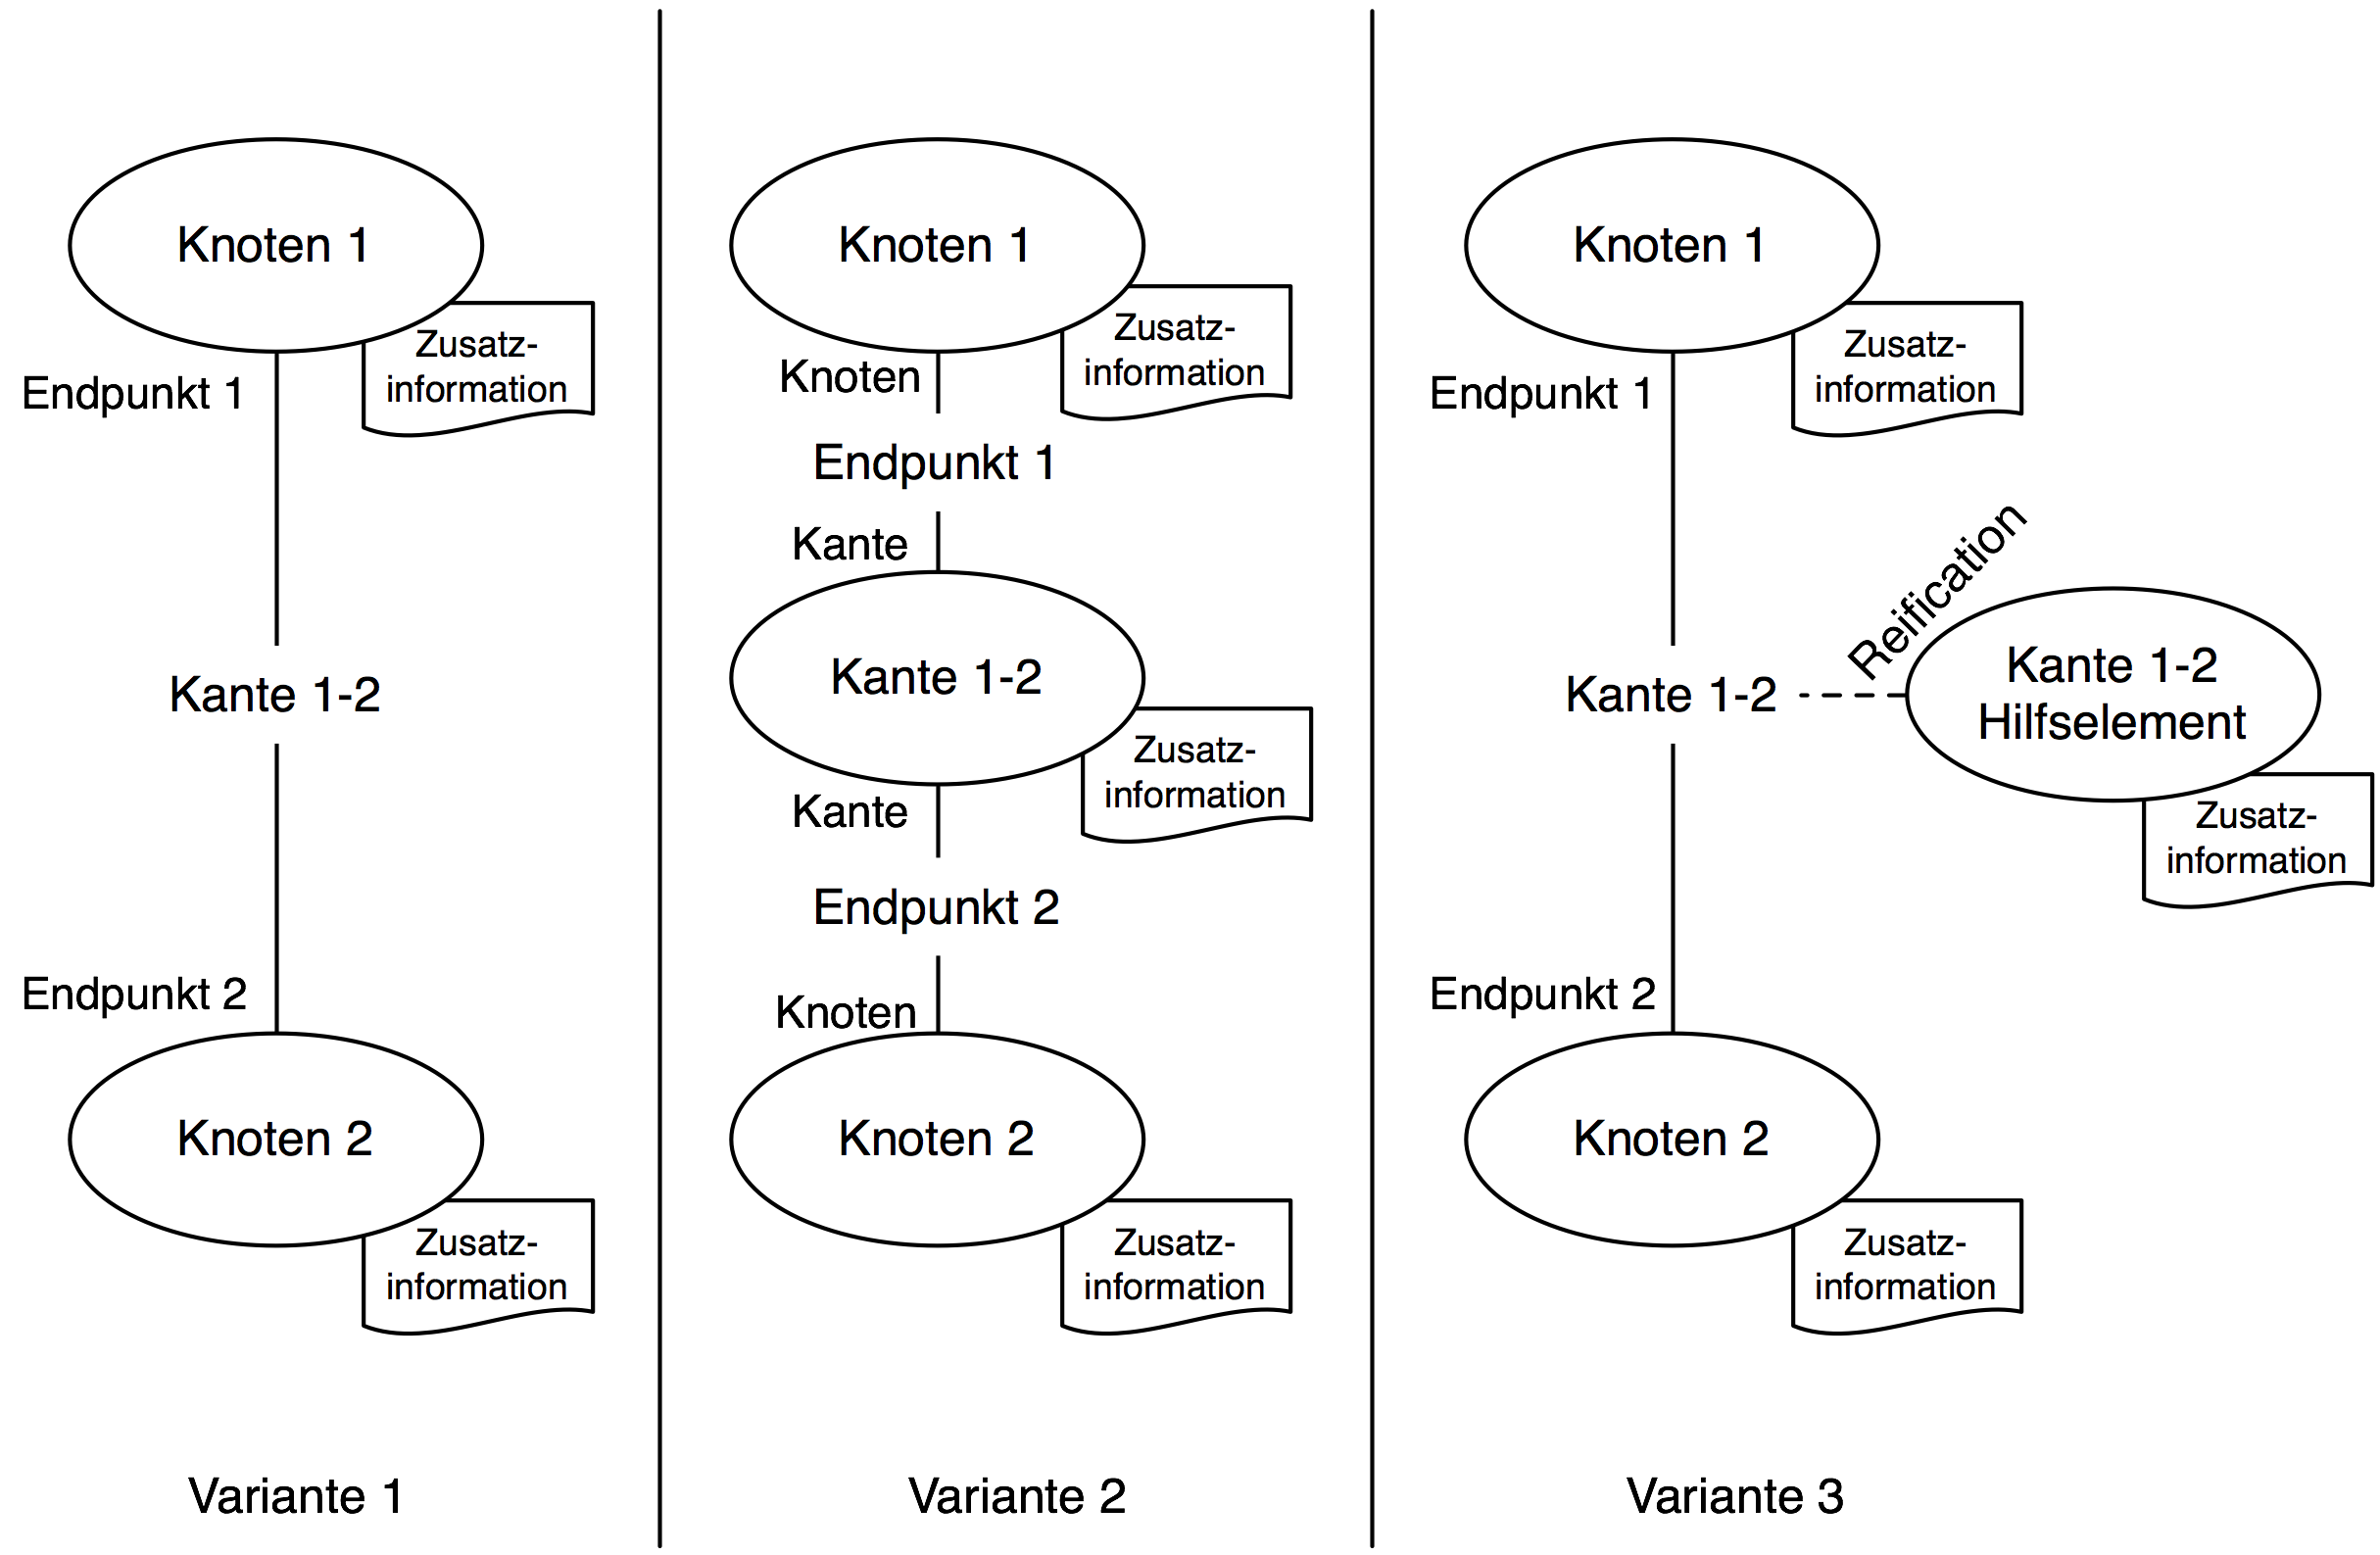
\includegraphics[width=13cm]{img/Persistenz/AssociationReification.png}
	\caption{Abbildung von Modellinformation in Topic Maps}
	\label{fig:img_Persistenz_AssociationReification}
\end{figure}

Die Bedeutung der Knoten des abzubildenden Modells im Kontext einer bestimmten Kante muss in den direkt abbildenden Varianten (in denen Kanten auf Associations abgebildet werden) durch Roles dargestellt werden. In der indirekten Abbildung (bei der Kanten auf Topics abgebildet werden), kann diese Information auch in den Associations repräsentiert werden, die die Topics die Knoten darstellen und jene die Kanten darstellen miteinander verbinden.
% subsection grundlegende_abbildung (end)

\subsection{Abbildung des Metamodells}
\label{sub:abbildung_des_metamodells}
Da Topic Maps von vorne herein nicht auf eine bestimmte semantische Bedeutung der Topics und Associations festgelegt sind, muss auch das Meta-Model der abgebildeten Modellierungssprache mit eingebettet werden. Dies wird in Topic Maps durch die Einbindung von Types ermöglicht. In den nun folgenden Ausführungen wird nur noch auf die direkt abbildende Variante Bezug genommen, da deren Ausdrucksstärke durch die Möglichkeit zur Reification gegenüber dem indirekt abbildenden Ansatz nicht eingeschränkt ist und die unmittelbare Abbildung zu insgesamt kleineren, einfacher zu verwaltenden Topic Maps führt (für eine Kanten wird nur eine Association benötigt, im Gegensatz dazu benötigt der alternative Ansatz ein Topic und mindestens zwei Associations zu Abbildung einer Kante).

Die in der Modellierungssprache festgelegten Arten von Knotentypen (also den eigentlichen Modellierungselementen) werden auf Topic Types abgebildet. Durch die Referenzierung eines einen Knoten repräsentierenden Topics auf diesen Topic Type wird die Bedeutung zugewiesen.

Ebenso wird mit Kanten verfahren. Durch die Einführung von Topics die als Association Types und Role Types fungieren, kann die Bedeutung einer Kante im abzubildenden Modell definiert werden. Dazu wird ein Association Type festgelegt, der die eigentliche Bedeutung der Kante festlegt, die zugehörigen Role Types definieren, wie viele Endpunkte existieren und welche Bedeutung diese haben. Für eine konkrete Kante wird dann eine Association und eine der Anzahl der Endpunkte entsprechende Nummer an Roles erstellt, denen der jeweilige Association bzw. Role Type zugewiesen wird. 

Die Verwendung von Occurrences und dementsprechend die Erstellung von Occurrence Types ist zur reinen Abbildung von diagrammatischen Modellen nicht notwendig. Die Verwendung von Occurrences kann aber sinnvoll sein, wenn aus dem ursprünglichen Modell ebenfalls Ressourcen referenziert werden, die für die weitere Verarbeitung des Modells notwendig sind. Occurrences werden dann im Sinne der Topic Map zur Referenzierung dieser Ressourcen verwendet, wobei sich die zu verwendenden Occurrence Types an der Bedeutung der Ressourcen im abzubildenden Modell orientiert.

Wie in Abschnitt \ref{sub:metamodellierung_in_topic_maps} bereits beschrieben, bietet die Topic Map selbst jedoch keine Möglichkeit, eine explizite Zuordnung zwischen Topic Types, Association Types und Role Types zu definieren, so dass ein in einer Topic Map repräsentiertes Modell auf semantische Korrektheit hin überprüft werden kann. Die einzige ohne zusätzliche Information überprüfbaren Bedingungen sind die Prüfungen, ob alle Knoten und Kanten (also Topics, Associations und Roles) einer Kategorie (also einem Type) zugewiesen  wurden.

Zusätzlich muss also eine externe Möglichkeit geschaffen werden, semantische Korrektheits-Bedingungen zu formulieren und zu überprüfen:
\begin{enumerate}
 \item Zulässige Kategorien von Knoten (Topic Types)
 \item Zulässige Kategorien von Kanten (Association Types, Role Types und eine Zuordnung zwischen diesen, die eine Aussage über die Anzahl und Bedeutung der Endpunkte der Kante zulässt)
 \item Zulässige Verbindungen zwischen Knoten und Kanten (Zuordnung zwischen Endpunkten einer Kantenkategorie und den Knotenkategorien, die diese Endpunkte belegen dürfen -- also eine Zuordnung zwischen Role Types und Topic Types)
\end{enumerate}

Wie bereits oben beschrieben, können derartige Bedingungen innerhalb oder außerhalb der Topic Map formuliert werden. Die Interpretation der formulierten Bedingungen und deren Anwendung auf konkrete Anwendungsfälle muss immer von außerhalb der Topic Map durchgeführt werden. Hier wird der Ansatz der Repräsentation der Bedingungen innerhalb der Topic Map verfolgt, um durch die Übermittlung einer Topic Map nicht nur ein Modell an sich zu übertragen sondern auch jene Information zu liefern, die zur Interpretation derselben notwendig ist.

Die Formulierung der Bedingungen erfolgt auf Ebene der als Types eingesetzten Topics und vervollständigt so das in der Topic Map enthaltene Meta-Modell der Sprache in der das zu repräsentierende Modell erstellt wurde. Die Information über zulässige Knoten und Kanten wird über die Festlegung von entsprechenden Types definiert. Für jeden Typen wird ein Topic eingeführt, das aus dem auf die Topic Map abgebildeten Modell referenziert werden kann. Alle oben notwendigen Zuordnungen zwischen diesen Types werden über Associations abgebildet, die die als Types verwendeten Topics verbinden (siehe Abbildung \ref{fig:img_Persistenz_MetaModelDef}).

\begin{figure}[htbp]
	\centering
		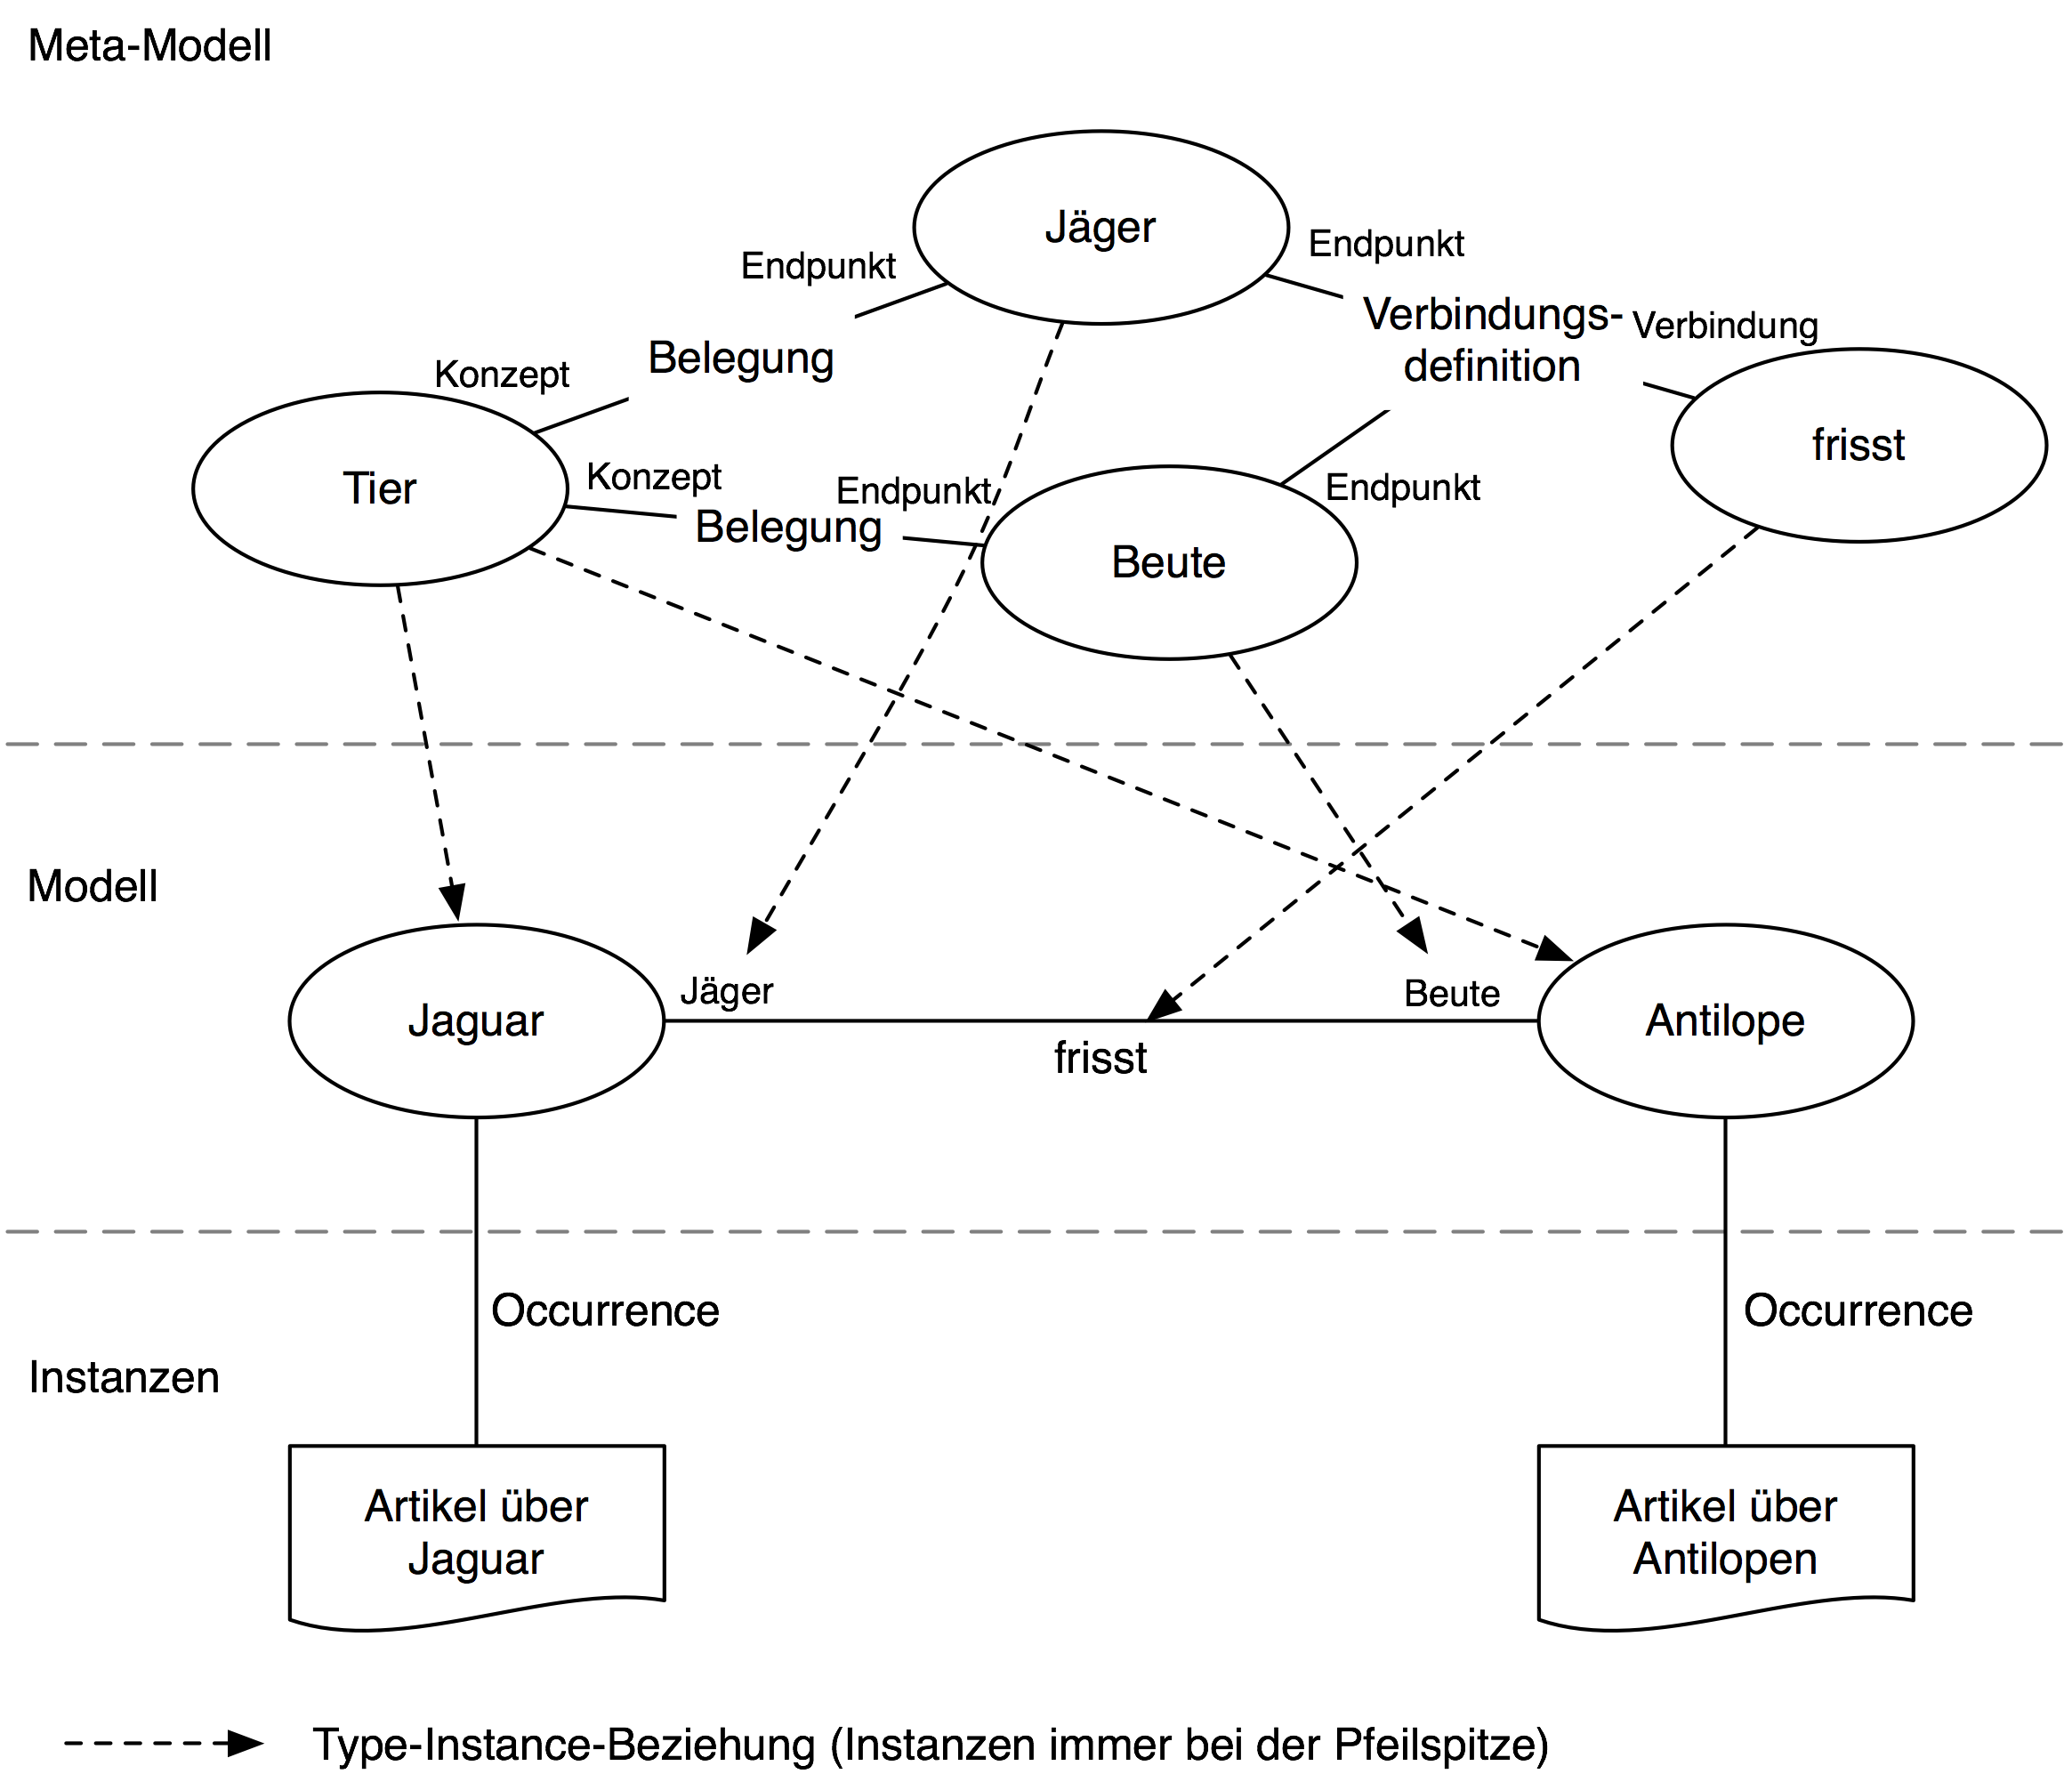
\includegraphics[width=13cm]{img/Persistenz/MetaModelDef.png}
	\caption{Definition des Meta-Models (ohne Kardinalitäten)}
	\label{fig:img_Persistenz_MetaModelDef}
\end{figure}

Die Definition der Kantentypen erfolgt über eine Association mit mindestens drei Roles. 
Eine dieser Roles referenziert den Association Type, die anderen Roles verweisen auf die zu verwendenden Role Types, die zur Beschreibung der Endpunkte der Kante verwendet werden (wovon mindestens zwei vorhanden sein müssen). Die Angabe der Kardinaliät (d.h. wie oft ein bestimmter Endpunkt im konkreten Modell auftreten darf) wird durch eine die jeweilige Role reifizierendes Topic festgelegt.

Ähnlich wird die Zuordnung zwischen Endpunkten und Knotenkategorien realisiert. Zwischen den entsprechenden Topic Types und Role Types werden Associations erstellt, die festlegen, ob eine bestimmte Knotenkategorie einen Endpunkt einnehmen darf oder nicht. Dazu enthält die betreffende Association mindestens zwei Roles, von denen eine auf den Role Type verweist, der den Endpunkt realisiert und eine entsprechende Anzahl von Roles, an die die zulässigen Topic Types (also Knotenkategorien) angebunden werden.

Die eben beschriebenen Abbildungsvorschriften selbst werden ebenfalls in der Topic Map abgebildet. Die Topic Map enthält damit auch das Meta-Meta-Modell das die Elemente die zur Festlegung eines Meta-Models und deren Zusammenspiel festlegt. Eine so definierte Topic Map ist also semantisch vollständig definiert und ermöglicht eine Rekonstruktion eines Modells, das in einer im Vorfeld unbekannten Sprache modelliert wurde, sofern lediglich das Meta-Meta-Modell bekannt ist, dass zur Interpretation der Sprachbeschreibung (Meta-Modell) notwendig ist (siehe Abbildung \ref{fig:img_Persistenz_MetaMetaModelDef}).

\begin{figure}[htbp]
	\centering
		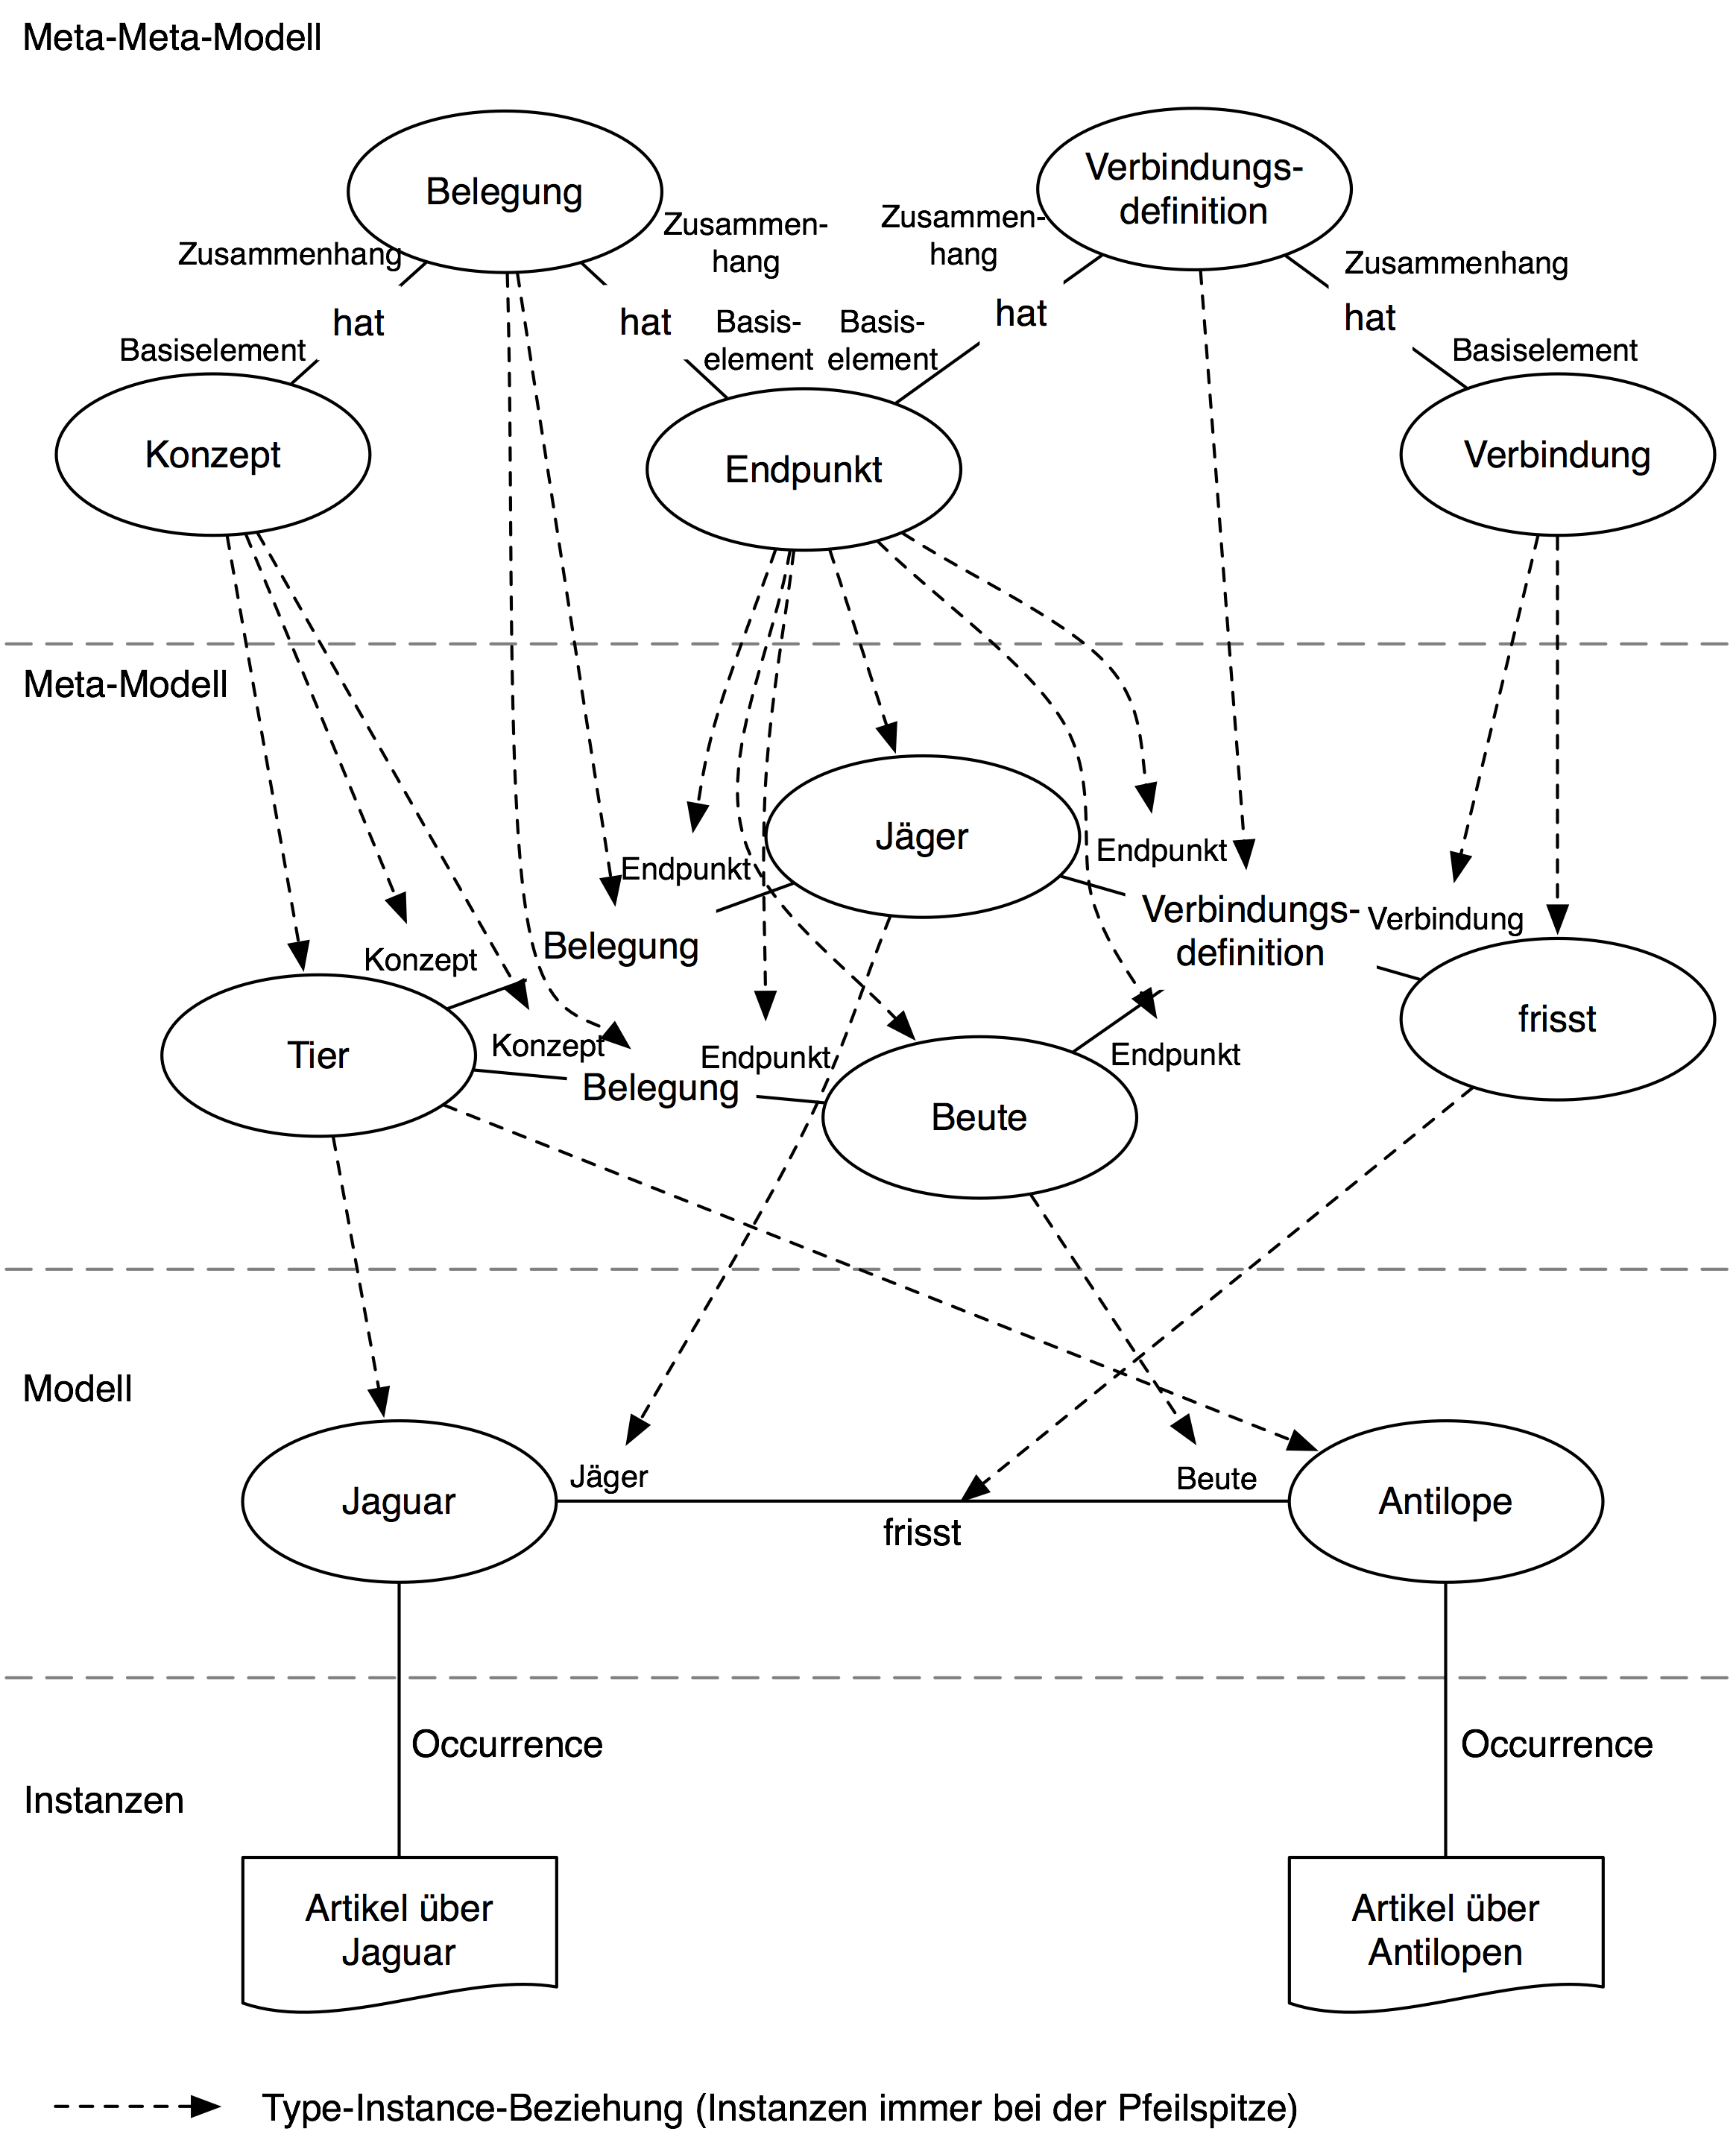
\includegraphics[width=13cm]{img/Persistenz/MetaMetaModelDef.png}
	\caption{Einbindung des Meta-Meta-Modells}
	\label{fig:img_Persistenz_MetaMetaModelDef}
\end{figure}

% subsection abbildung_des_metamodells (end)

\subsection{Abgrenzung von Submodellen}
\label{sub:abgrenzung_von_submodellen}

In einem Modell kann es sinnvoll oder notwendig sein, unterschiedliche Modellbereiche voneinander abzugrenzen. Der Grund für die Abgrenzung kann ein inhaltlicher sein (z.B. eine Partitionierung nach Akteuren bei Aktivitätsdiagrammen \citep{Rumbaugh04}) oder aus dem Modellierungsvorgang heraus motiviert sein (etwa bei der Abgrenzung von Teilmodellen, die durch verschiedene Personen erstellt wurden). Außerdem ist es möglich, in einer Topic Map mehrere Modelle zu repräsentieren, die ebenfalls voneinander abgrenzt werden müssen.

Für diese Abgrenzung bietet sich die Verwendung von Scopes an. Scopes haben zwar keinen Einfluss auf die vorhandenen Topics, wirken jedoch auf die Statements und -- hier relevant -- vor allem auf die die Topics verbindenden Associations. Werden also Scopes eingesetzt, um Teilmodelle voneinander zu unterscheiden bzw. zu trennen, so können die im Moment nicht relevanten Teilmodelle zwar nicht „ausgeblendet“ werden (im Sinne von „temporär vollkommen entfernt“, durch die Entfernung der nicht relevanten Statements sind jedoch nur noch jene Topics untereinander verbunden, die dem aktuell betrachteten Submodell angehören. Ausgehend von einer beliebigen, im Scope gültigen Association oder einem Topic, das bekannterweise dem aktuellen Teilmodell angehört kann so der gesamte relevante Teil der Topic Map erschlossen werden.

Die Realisierung der Trennung zwischen Teilmodellen durch das Ausblenden irrelevanter Verbindungen zwischen Topics birgt einen weiteren potentiellen Vorteil. Werden in einer Topic Map mehrere untereinander zusammenhängende Modelle abgebildet, so wird -- der Grundforderung einer Topic Map nach Eineindeutigkeit entsprechend -- jedes Element nur einmal abgebildet, egal ob es in nur einem Modell verwendet wird oder in mehreren. Durch den Einsatz von Scopes bilden in mehreren Modellen verwendete Elemente automatisch eine Schnittstelle, an der zwischen den Modellen navigiert werden kann. Dieser Vorteil muss in herkömmlichen Modellierungsansätzen mit mehreren untereinander verknüpften Modellen wie der \gls{UML} \citep{Rumbaugh04} oder ARIS \citep{Scheer03} technisch durch explizite Verknüpfung bzw. Referenzierung der äquivalenten Modellelemente in den unterschiedlichen Modeller erzeugt werden. 

Zur Kennzeichnung des Scopes muss zumindest ein Topic verwendet werden. Im Meta-Modell muss festgelegt werden, ob dazu ein Topic eines bestehenden Types verwendet wird oder ein neuer Type eingeführt werden, dessen Topics ausschließlich zum Aufspannen eines Scopes verwendet werden. Dazu wird im Meta-Meta-Modell ein Type „Partition“ eingeführt, der der für alle Elemente des Meta-Modells verwendet werden muss, deren konkrete Instanzen einen Scope im Modell kennzeichnen sollen.

% subsection abgrenzung_von_submodellen}

\subsection{Flexibilisierung der Abbildung}
\label{sub:flexibilisierung_der_abbildung}

Wie in Kapitel XY beschrieben, ist das Meta-Modell von Modellen die im vorgestellten Ansatz entstehen, nicht im vorhinein festgelegt. Die Modellierungssprache -- also das Meta-Modell -- wird während der Modellbildung semantisch definiert und ist damit erst zur Modellierungszeit bekannt. Das Metamodell kann außerdem während der Modellierung erweitert werden, es ist auch möglich, dass sich die Bedeutung bereits existierender Meta-Modell-Elemente ändert.

Für die Persistierung bedeutet dies, dass das Meta-Modell nicht im Vorhinein sondern erst zum Zeitpunkt der Speicherung festgeschrieben werden kann. Außerdem kann die Prüfung auf semantische Korrektheit des Modells ebenfalls nur durchgeführt werden, sobald das Modell definiert ist. 

Um die geforderte Flexibilität bei der Sprachdefinition in Form und Zeitpunkt zu gewährleisten, wurde von \citet{Neubauer08} ein System entwickelt, dass es erlaubt, dynamisch zur Laufzeit Modellelemente zu definieren, die Regeln zu deren Verwendung festzulegen und diese ohne Unterbrechung des Modellierungsvorgangs unmittelbar zu verwenden (wobei auch die Prüfung der semantischen Korrektheit zur Laufzeit adaptiert wird). Die technische Umsetzung dieses Ansatzes wird in Abschnitt \ref{sec:dynamische_metamodelle} beschrieben.

% subsection flexibilisierung_der_abbildung (end)

% section abbildung_von_modellen_auf_topic_maps (end)

\section{Technische Umsetzung der Persistierung von Modellen} % (fold)
\label{sec:technische_umsetzung_der_persistierung_von_modellen}

Die oben beschriebenen Konzepte zur Persisitierung von Modellen wurden wie die übrigen Software-Komponenten des Systems in Java implementiert. Die Basis der Persistenz-Komponente bildet eine Topic Map Engine, die im Rahmen einer Arbeit über flexible Content-Repräsentation vom Autor entwickelt wurde \citep{Oppl07}. Das in \citep{Neubauer08} entwickelte System zur Generierung und Verwendung dynamischer Metamodelle, das bereits in Abschnitt \ref{sub:flexibilisierung_der_abbildung} konzeptuell beschrieben wurde, wird in der Folge hinsichtlich seiner technischen Umsetzung betrachtet. Basierend auf diesen beiden Komponenten wurde die eigentlichen Persistierung implementiert. Der dort verfolgte Ansatz ist Thema des letzten Teils dieses Abschnitts.

\subsection{Topic Map Engine}

Als Topic Map Engine bezeichnet man ein Software-Modul, mit dessen Hilfe Topic Maps verwaltet werden können und das im Normalfall auch Funktionalität zur Persistierung der Topic Map anbietet. Für den Topic Map Standard REF, der dieser Arbeit zugrunde liegt, war zum Zeitpunkt der Erstellung der Software nur eine derartige Engine vertrieben, die von Ontopia\footnote{http://www.ontopia.com} kommerziell vertrieben wird und keine offenen Schnittstellen bietet. Zu diesem Zeitpunkt noch nicht für den verwendeten Topic Map Standard verfügbar war die Open-Source-Engine TinyTIM\footnote{http://???}, die auf Basis der ebenfalls erst seit einigen Monaten verfügbaren Topic Map \gls{API} eine offene Schnittstelle zur Verwaltung von Topic Maps in Java anbietet und unterschiedliche Formate zur Persistierung und zum Import unterstützt.

Für diese Arbeit wurde mangels verfübarer Alternativen eine eigene Topic Map Engine erstellt, deren Funktionalität und Aufbau hier nur kurz umrissen werden soll. Die detaillierte Beschreibung der Implementierung und die allgemeine Verwendung der Engine sind in \ref{Oppl07} beschrieben.

\subsubsection{Kernkomponenten}

Die Topic Map Engine bildet die Komponenten einer Topic Map direkt auf Java Klassen ab.

\subsubsection{Einführung von Domänenmodellen}

\subsubsection{Schnittstelle zur Persistierung}

Die Topic Map Engine bietet zur Persistierung ein einfaches Interface an, über welches Topic Maps auf der Engine exportiert werden können bzw. in die Engine geladen werden. Das Interface abstrahiert dabei von der konkreten Persistierungs-Technologie und erlaubt die Einbindung unterschiedlicher Ansätze zur Speicherung von Topic Maps.

Konkret wurden drei Implementierungen des Persistenz-Interfaces erstellt. Die erste Implementierung liest und schreibt Topic Maps von bzw. in im \gls{XTM}-Format REF abgelegten \gls{XML}-Dateien. So wird ein standardkonformer Datenaustausch zwischen Topic Map Engines ermöglicht. Die zweite Implementierung bindet die Topic Map Engine via Hibernate REF an eine relationale Datenbank an. Im Gegensatz zur Speicherung in XML-Files ermöglicht die Ablage der Daten in einem RDBMS einen effizienteren, selektiven Zugriff, sodass nicht unter allen Umständen die gesamte Datenbasis einer Topic Map im Arbeitsspeicher gehalten werden muss.

Die dritte Implementierung des Persistenz-Interfaces ermöglicht lediglich den Export einer Topic Map in ein von GraphViz REF interpretierbares Format, das eine graphische Darstellung der Topic Map mit automatische Anordnung der Topics ermöglicht. Da das GraphViz-Format jedoch nicht so ausdrucksstark ist wie der Topic Map Ansatz, geht beim Export Information verloren. Dadurch ist es nicht möglich, eine Topic Map aus einem GraphViz-File zu rekonstrieren, der Import in die Engine ist also nicht möglich. 

\begin{figure}[htbp]
	\centering
		\includegraphics[width=10cm]{img/Persistenz/GraphVizExample.jpg}
	\caption{Ausschitt einer mittels GraphViz visualisierten Topic Map}
	\label{fig:img_Persistenz_GraphViz}
\end{figure}

Zusätzlich zur Ausgabe der gesamten Topic Map ist das GraphViz-Export-Modul auch in der Lage eine mittels HTML Imagemaps navigierbare Version der Topic Map zu exportieren, in der jeweils immer nur ein Topic mit dessen Kontext (also allen Topics, die mit dem zentralen Topic verbunden sind) dargestellt wird (siehe Abbildung XY). Durch die Imagemap werden die Kontext-Topics mit jenen Ansichten verknüpft, wo jeweils diese im Fokus der Betrachtung stehen. Damit ist eine schrittweise Navigation durch die Topic Map möglich.

\subsection{Dynamische Metamodelle}
\label{sec:dynamische_metamodelle}

\subsection{Persistierung}
% section technische_umsetzung_der_persistierung_von_modellen (end)


\section{Export graphischer Repräsentationen} % (fold)
\label{sec:export_graphischer_repräsentationen}

Neben der Persistierung der Modelle in Form einer Topic Map ist es auch sinnvoll, die Modelle in deren graphischer Form als Referenz abzulegen. Das hier entwickelte Werkzeug bedient sich der graphischen Ausgabefunktionalitäten, die der Java Klassenbibliothek mit der Version 1.4 hinzugefügt wurden, um das aktuelle Modell in unterschiedlichen Formen als Grafik auszugeben und zur späteren Referenz zu speichern.

\subsection{Ausgabeformen} % (fold)
\label{sub:ausgabeformen}

Zur Speicherung der graphischen Repräsentation eines Modells wird grundsätzlich die Visualisierung verwendet, die auf dem sekundären Ausgabekanal (also dem Bildschirm) zur Anwendung kommt. Beim Export sind nun unterschiedliche Modellaspekte zu berücksichtigen, die je nach intendiertem Verwendungszweck einzeln oder in Kombination in die Ausgabe eingehen können. Diese Aspekte sind im Einzelnen
\begin{itemize}
	\item der aktuell auf der Oberfläche befindliche Modellzustand
	\item die hierarchisch in diesen eingebetteten Submodelle
	\item die Modellierungshistorie, also die Entwicklung des Modells über die Zeit
\end{itemize}

Die Darstellung dieser Aspekte in einer graphischen Repräsentation ist (außer im erstgenannten Fall) insofern komplex, als dass eine beliebig lange zeitliche Abfolge bzw. eine beliebig tief verschachtelte Hierarchie in den zweidimensionalen Raum abgebildet werden muss. Im Falle einer Kombination des zweit- und drittgenannten Aspektes müssen zwei Dimensionen zugleich abgebildet werden, was die Darstellung zusätzlich erschwert.

Der aktuell auf der Oberfläche befindliche Modellzustand wird exakt wie dargestellt in eine Grafik transformiert und als Bild abgespeichert. Zur Abbildung der Modellierungshistorie bietet sich an, die einzelnen gespeicherten Modellzustände chronologisch anzuordnen. Der sich so ergebende Zeitstrahl beginnt links oben und setzt sich von links nach recht und oben nach unten bis in die rechte untere Ecke fort, wo wiederum der aktuelle Modellzustand dargestellt wird. Die zweidimensionale Abbildung des Zeitstrahls erfolgt dabei derart, das sowohl die horizontale als auch die vertikale Ausdehnung des resultierenden Bildes minimal sind (siehe Abbildung \ref{fig:img_Persistenz_ExportHistorie}).

\begin{figure}[htbp]
	\centering
		\includegraphics[width=15cm]{img/Persistenz/ExportHistorie.png}
	\caption{Modellierungshistorie als exportierte Grafik}
	\label{fig:img_Persistenz_ExportHistorie}
\end{figure}

Bei der Darstellung eines Modells mit hierarchisch geschachtelten Teilmodellen bietet sich eine baumartige Darstellung mit dem aktuellen Modellzustand als Wurzelknoten an. Diese ist aufgrund der notwendigen Detaildarstellung der einzelnen Modelle jedoch platzintensiv und kann nur schwer als physisches Dokument abgelegt werden. Deshalb wurde alternativ die hierarchische Struktur auf eine der Darstellung der zeitlichen Modellentwicklung ähnliche Darstellungsform abgebildet. Dabei wird die Hierarchie flach ausgerollt, die Einbettungen zeigen sich durch einen graduell dunkler werdenden Modellhintergrund für tiefere verschachtelte Ebenen. Zusätzlich wird in jedes Submodell farblich abgesetzt auch das jeweilige Containerelement eingeblendet. Die Abfolge der einzelnen Modelle startet mit dem aktuellen Modellzustand als erstem Knoten. Dahinter wird das erste im aktuellen Modell eingebettete Teilmodell angezeigt. Besitzt dieses Teilmodell wiederum eingebettete Teilmodelle, so werden diese in der Folge mit erneut abgedunkeltem Hintergrund dargestellt. Diese Form der Darstellung wird fortgesetztm bis keine weiteren eingebetteten Modelle mehr vorhanden sind. Es folgt (sofern vorhanden) das zweite Submodelle des aktuellen Modellzustandes (mit dem abgedunkelten Hintergrund der ersten Einbettungsebene). Diese Hierarchie wird wiederum bis zu den Endpunkten nach unten verfolgt, es folgt ggf. das dritte Submodell auf der ersten Einbettungsebene. Die sich so ergebende Linie an Modellzuständen wird wie der chronologischen Darstellung der Modellierungshistorie so umgebrochen dass sich sowohl in horizontaler als auch in vertikaler Richtung eine minimale Ausdehung ergibt (siehe Abbildung \ref{fig:img_Persistenz_ExportHierarchie}).

\begin{figure}[htbp]
	\centering
		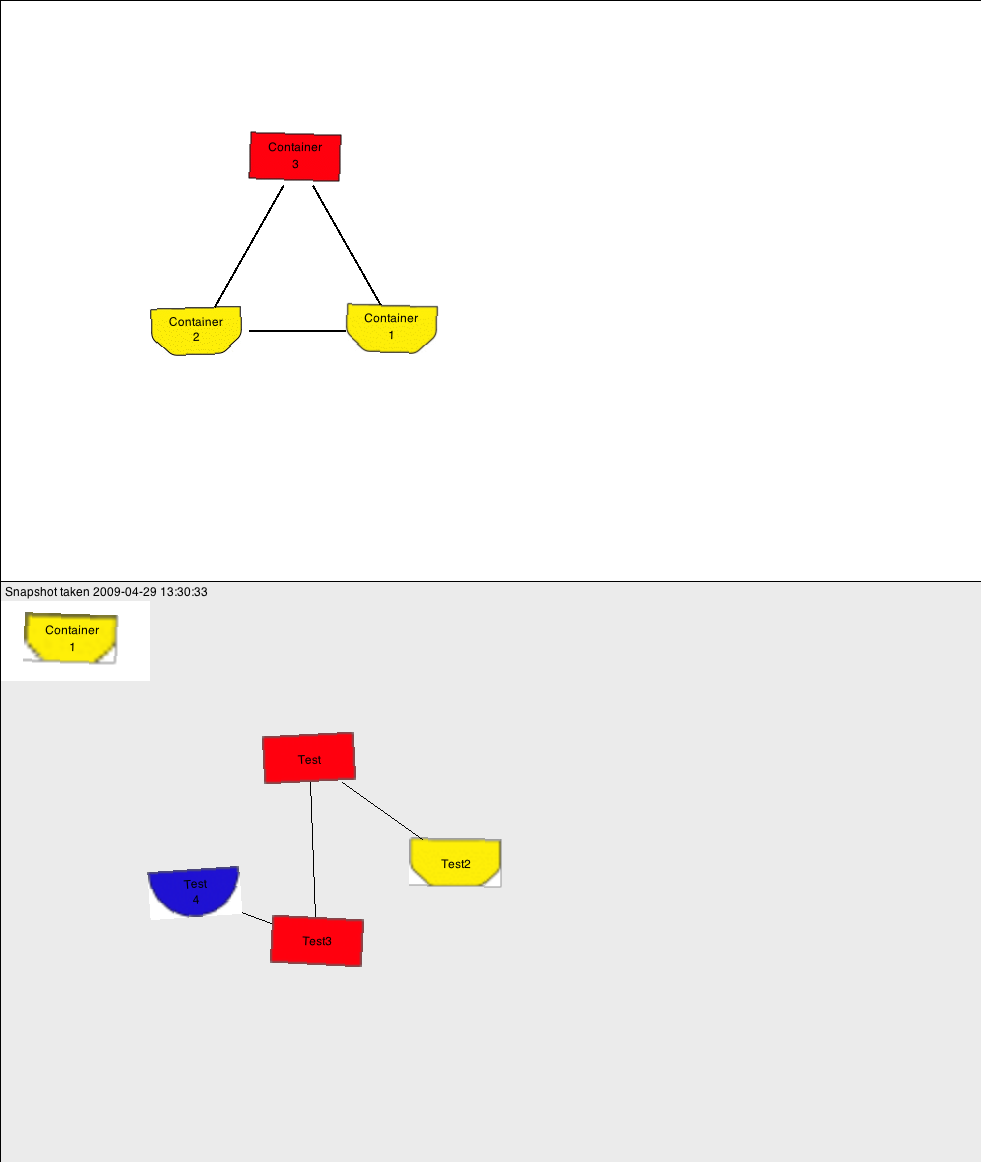
\includegraphics[width=15cm]{img/Persistenz/ExportHierarchie.png}
	\caption{Modell-Hierarchie als exportierte Grafik}
	\label{fig:img_Persistenz_ExportHierarchie}
\end{figure}

In der komplexesten Ausprägung der Darstellung eines Modells als graphische Repräsentation werden sowohl die Historie der Modellentstehung als auch die Hierarchie der eingebetteten Submodelle zugleich dargestellt. Dies erfolgt hier durch die Kombination der beiden eben beschriebenen Ansätze. Die Darstellung der Modellierungshistorie bildet die oberste Ebene der Modelldarstellung. Beginnend mit dem ältesten gespeicherten Modellzustand werden die einzelnen Modelle in der Reihenfolge ihrer Entstehung abgebildet, wobei zu jedem Modellzustand unmittelbar folgend dessen eingebetteten Submodelle ausgegeben werden (deren Entstehung nicht mehr separat dargestellt wird). So ergibt sich eine kombinierte Linie aus chronologischer Modellentwicklung und eingebetteten Teilmodellen. Diese wird wie schon oben mit minimaler Ausdehnung in horizontaler wie vertikaler Richtung auf eine Grafik abgebildet. Die Entwicklung des Modells ist dabei wie gehabt von links oben nach rechts unten zu verfolgen, wobei nur jene Modellzustände mit weißem Hintergrund auf oberster Ebene der Zeitlinie angehören. Alle dunkler hinterlegten Modelle sind Teilmodelle und sind dem nach vorne nächstgelegenen weiß hinterlegten Modell zuzuordnen.

% subsection ausgabeformen (end)

\subsection{Technische Umsetzung des graphischen Exports} % (fold)
\label{sub:technische_umsetzung_des_graphischen_exports}

Zur Umsetzung des graphischen Exports wird auf die mit der Java Plattform in der Version 1.4 eingeführten Klassen zu Verarbeitung von Grafikformaen zurückgegriffen. Diese unterstützen standardmäßig gängige Grafikformate wie \gls{JPEG}, \gls{GIF} oder \gls{PNG}. Im konkreten Fall wurde ein verlustfrei komprimierendes Format gewählt, verlustbehaftete Verfahren wie \gls{JPEG} sind für die hier abzubildenden feinen Strukturen nicht geeignet, da es durch Kompressionsartefakte zu Qualitätsminderungen in der Darstellung von Details kommt.

Die Ausgabe einer Datei im gewählten Grafikformat wird vollständig von der Klasse \texttt{ImageIO} übernommen. Der Schnittstellen-Methode \texttt{write} sind als Parmeter der Dateiname, das Grafikformat sowie ein Objekt der Klasse \texttt{BufferedImage} (allgemeiner: einer Klasse, die das Interface \texttt{RenderedImage} implementiert) zu übergeben, dass die eigentlichen Bilddaten enthält.

Das \texttt{BufferedImage}-Objekt kann durch einen Methoden-Aufruf mit der graphischen Repräsentation einer Klasse, die von der Java \gls{AWT}-Klasse \texttt{Component} abgeleitet ist, befüllt werden. Da alle graphischen Komponenten des JHotDraw-Frameworks Subklassen eben dieser Klasse sind (inklusive der Zeichenoberfläche selbst), können diese durch einen Aufruf ihrer \texttt{paint}-Methode in ein ausreichend großes \texttt{BufferedImage} (bzw. dessen \texttt{Graphics}-Objekt) geschrieben werden.  

In den aus mehr als einem Teilmodell bestehenden Ausgaben (also der Historie, der hierarchischen Darstellung der Teilmodelle oder der Kombination dieser beiden Fälle) muss das Bild aus den graphischen Repräsentationen der einzelnen Teilmodelle zusammengesetzt werden. Dazu werden (im Falle der hierarchischen Teilmodelle rekursiv) die logischen Modelle erzeugt und bereits in der korrekten linearisierten Darstellungsform in einem \texttt{Vektor} gespeichert. Die einzelnen logischen Modelle werden dann in graphische Repräsentationen umgewandelt und in je einem \texttt{BufferedImage} gespeichert. Diese werden in der Folge so zusammengesetzt, dass die horizontale und vertikale Ausdehung der Gesamtfläche minimal ist.

% subsection technische_umsetzung_des_graphischen_exports (end)
% section export_graphischer_repräsentationen (end)

\section{Zusammenfassung} % (fold)
\label{sec:persistierung_zusammenfassung}

% section persisitierung_zusammenfassung (end)
% chapter persistierung (end)
